% ===================================================================
% Team 07 - MME / Ichor Systems Universal Plastic Shredder V2.0
% ECE 412/413 Capstone Poster (Spring 2026)
% 48 x 36 in landscape, single page, PSU MCECS look
% ===================================================================
\documentclass[ansiE, landscape]{sciposter}
% Author notes the rendered top/left borders read visually bigger than
% the bottom/right ones (likely a sciposter + multicols quirk that adds
% slack inside the green title banner). Compensate by halving the top
% and left geometry margins so the visible borders look equal.
% Asymmetric geometry: left and top halved (twice) from the original
% 1.5 in to compensate for sciposter + multicols visual slack so the
% rendered borders read as equal.
\usepackage[paperwidth=48in,paperheight=36in,
            left=0in,right=2.25in,top=0in,bottom=1.5in]{geometry}
\setlength{\paperwidth}{48in}
\setlength{\paperheight}{36in}
\setlength{\textwidth}{45.75in}
\setlength{\textheight}{34.5in}
\setlength{\oddsidemargin}{-1in}
\setlength{\evensidemargin}{-1in}
\setlength{\topmargin}{-1in}
\setlength{\headheight}{0pt}
\setlength{\headsep}{0pt}
\setlength{\footskip}{0pt}
\setlength{\columnsep}{0.6in}

\usepackage{multicol}
\usepackage{color}
\usepackage{graphicx}
\usepackage{amsmath}
\usepackage{url}
\usepackage{textcomp}
\usepackage[skins,breakable,raster]{tcolorbox}
\usepackage{tikz}
\usepackage{adjustbox}

% PSU palette
\definecolor{PSUgreen}{RGB}{106,127,16}
\definecolor{PSUltgreen}{RGB}{168,180,0}
\definecolor{PSUblue}{RGB}{0,117,154}
\definecolor{PSUltblue}{RGB}{161,216,224}
\definecolor{PSUgray}{RGB}{71,67,52}
\definecolor{PSUred}{RGB}{210,73,42}
\definecolor{PSUorange}{RGB}{220,155,50}
\definecolor{PSUcream}{RGB}{250,247,238}

% Typography
\renewcommand{\LARGE}{\fontsize{96pt}{106pt}\selectfont}
\renewcommand{\Large}{\fontsize{58pt}{64pt}\selectfont}
\renewcommand{\large}{\fontsize{30pt}{36pt}\selectfont}
\renewcommand{\normalsize}{\fontsize{18pt}{22pt}\selectfont}
\renewcommand{\titlesize}{\LARGE}
\renewcommand{\authorsize}{\Large}
\renewcommand{\instsize}{\large}

% Empty out the default sciposter title -- we draw our own banner
\title{}
\author{}
\institute{}
\conference{}
\renewcommand{\footlogo}{}

% Custom section header: green pill with white text + tiny shadow line under
\newcommand{\postersec}[1]{%
  \par\vspace{6pt}%
  \noindent
  \begin{tcolorbox}[
    enhanced, sharp corners, boxrule=0pt, frame hidden,
    interior style={top color=PSUgreen, bottom color=PSUgreen!90!black},
    coltext=white,
    left=14pt, right=14pt, top=6pt, bottom=6pt,
    width=\linewidth,
    fontupper=\sffamily\bfseries\large,
    drop shadow=PSUgray!40,
  ]
  #1
  \end{tcolorbox}%
  \par\vspace{4pt}
}

% Wide colored cards inside a tcbraster (for the highlights strip)
\newtcolorbox{statcard}[1]{enhanced, sharp corners, boxrule=0pt, frame hidden,
  interior style={top color=PSUcream, bottom color=white},
  borderline north={3pt}{0pt}{PSUgreen},
  left=12pt, right=12pt, top=8pt, bottom=10pt,
  fontupper=\sffamily, title=#1, coltitle=PSUgreen,
  fonttitle=\sffamily\bfseries\large,
  attach title to upper={\par\smallskip}}

\begin{document}

% ============== TITLE BANNER (replaces default \maketitle) ==============
\noindent
\begin{tcolorbox}[
  enhanced, sharp corners, boxrule=0pt, frame hidden,
  interior style={top color=PSUgreen, bottom color=PSUltgreen},
  coltext=white,
  left=30pt, right=30pt, top=18pt, bottom=18pt,
  width=\textwidth,
  fontupper=\sffamily,
]
\begin{minipage}[c]{0.72\linewidth}
  {\fontsize{90pt}{96pt}\selectfont\bfseries
   UNIVERSAL PLASTIC SHREDDER V2.0}\\[6pt]
  {\fontsize{40pt}{46pt}\selectfont\bfseries Electrical Control \& Power System}\\[14pt]
  {\fontsize{28pt}{32pt}\selectfont
   Bao Nguyen\;\textbullet\;Fearghus Tyler\;\textbullet\;Yaqoub Rabiah\;\textbullet\;Fox Kang}\\[6pt]
  {\fontsize{22pt}{26pt}\selectfont
   Portland State University\,\textbullet\,MCECS\,\textbullet\,Department of Electrical \& Computer Engineering}\\[2pt]
  {\fontsize{22pt}{26pt}\selectfont
   Sponsor: MME / Ichor Systems (Bridget Lannigan)\quad\textbar\quad
   Advisors: Prof.~Andrew Greenberg, Dr.~Jonathan Bird (EE), Robert Paxton (ME)}
\end{minipage}\hfill
\begin{minipage}[c]{0.10\linewidth}
  \centering
  
\includegraphics[width=\linewidth]{./Pictures/QR_GitHub.png}\\[2pt]
  {\footnotesize\sffamily\bfseries Scan for the repo}
\end{minipage}\hfill
\begin{minipage}[c]{0.15\linewidth}
  \raggedleft
  \adjustbox{max width=\linewidth,max height=2.4in}{
\includegraphics{./Logo/psuMCECSloghoriz.png}}
\end{minipage}
\end{tcolorbox}

\vspace{12pt}

\begin{multicols}{3}

%================ COLUMN 1 ================
\postersec{The Problem}
\begin{itemize}\setlength{\itemsep}{2pt}
  \item Ichor Systems creates large volumes of thick rigid plastic waste (PVC, PP, LDPE) from semiconductor manufacturing.
  \item Sheets are 0.25--0.5\,in.~thick, 4--12\,in.~wide -- off-the-shelf shredders are too small or too expensive.
  \item Our scope: \textbf{electrical control + power system}. Mechanical frame and blades come from the ME team.
\end{itemize}

\postersec{Requirements}
\textbf{Must:}
\begin{itemize}\setlength{\itemsep}{2pt}
  \item Shred plastic to $\sim$1\,in.~pieces.
  \item Drive a 3--5\,HP motor at 70--90\,RPM through a controllable VFD.
  \item Follow NFPA 70 (NEC); include E-stop, overload, and one safety interlock.
  \item Provide an HMI for operator control and status.
  \item Stay within the \$1{,}000 EE-team budget.
\end{itemize}
\textbf{Should:} status / fault lights, NEMA enclosure, labeled controls. \\
\textbf{May:} read-only wireless monitoring, data logging, capacitive-touch safety.

\postersec{System Architecture}
\begin{itemize}\setlength{\itemsep}{2pt}
  \item \textbf{Industrial stack:} AutomationDirect end-to-end. No hobby boards in the control or safety path.
  \item \textbf{Power path:} PowerTec 71008 disconnect $\rightarrow$ Mean Well 24\,VDC PSU $\rightarrow$ SD-N35 contactor $\rightarrow$ Huanyang VFD $\rightarrow$ motor.
  \item \textbf{Motor:} IronHorse MTCP2-002, 2\,HP, 230\,V, 1735\,RPM, VFD-rated.
  \item \textbf{Safety:} E-stop hardwired through the contactor coil, parallel to the PLC.
\end{itemize}

\begin{center}
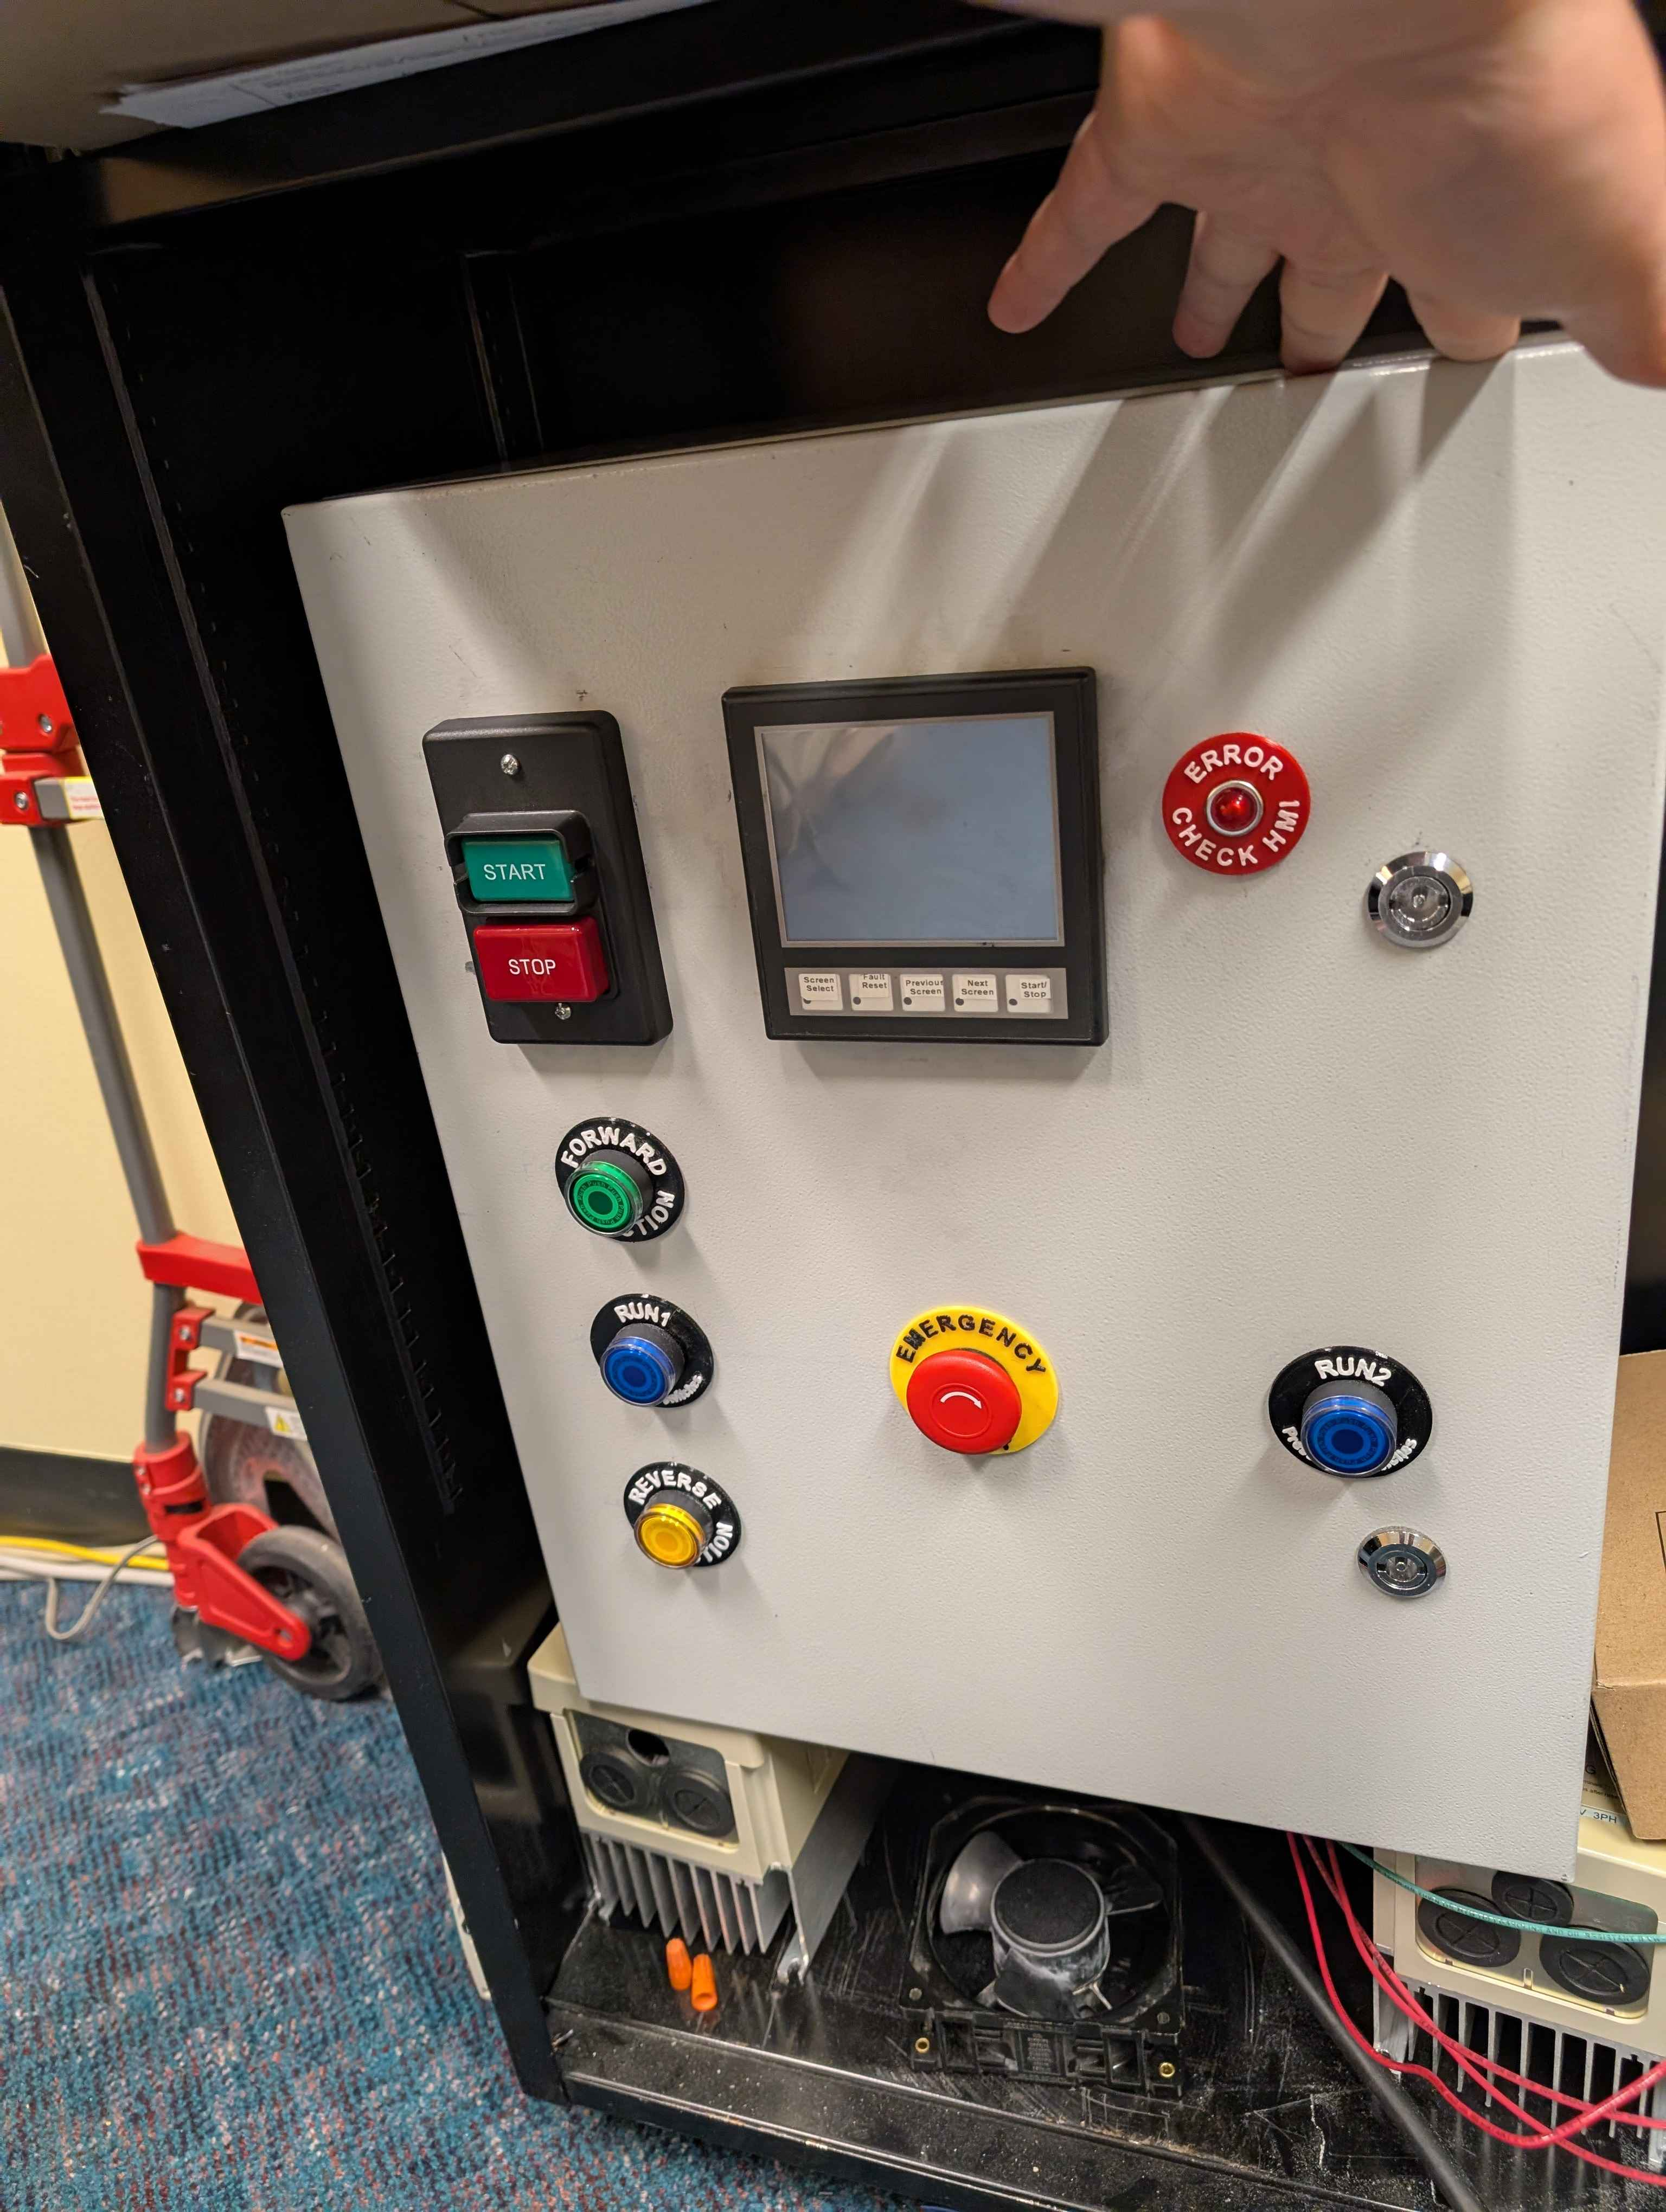
\includegraphics[height=6.5in]{./Pictures/Photo_Front_Panel.jpg}\hspace{3pt}%
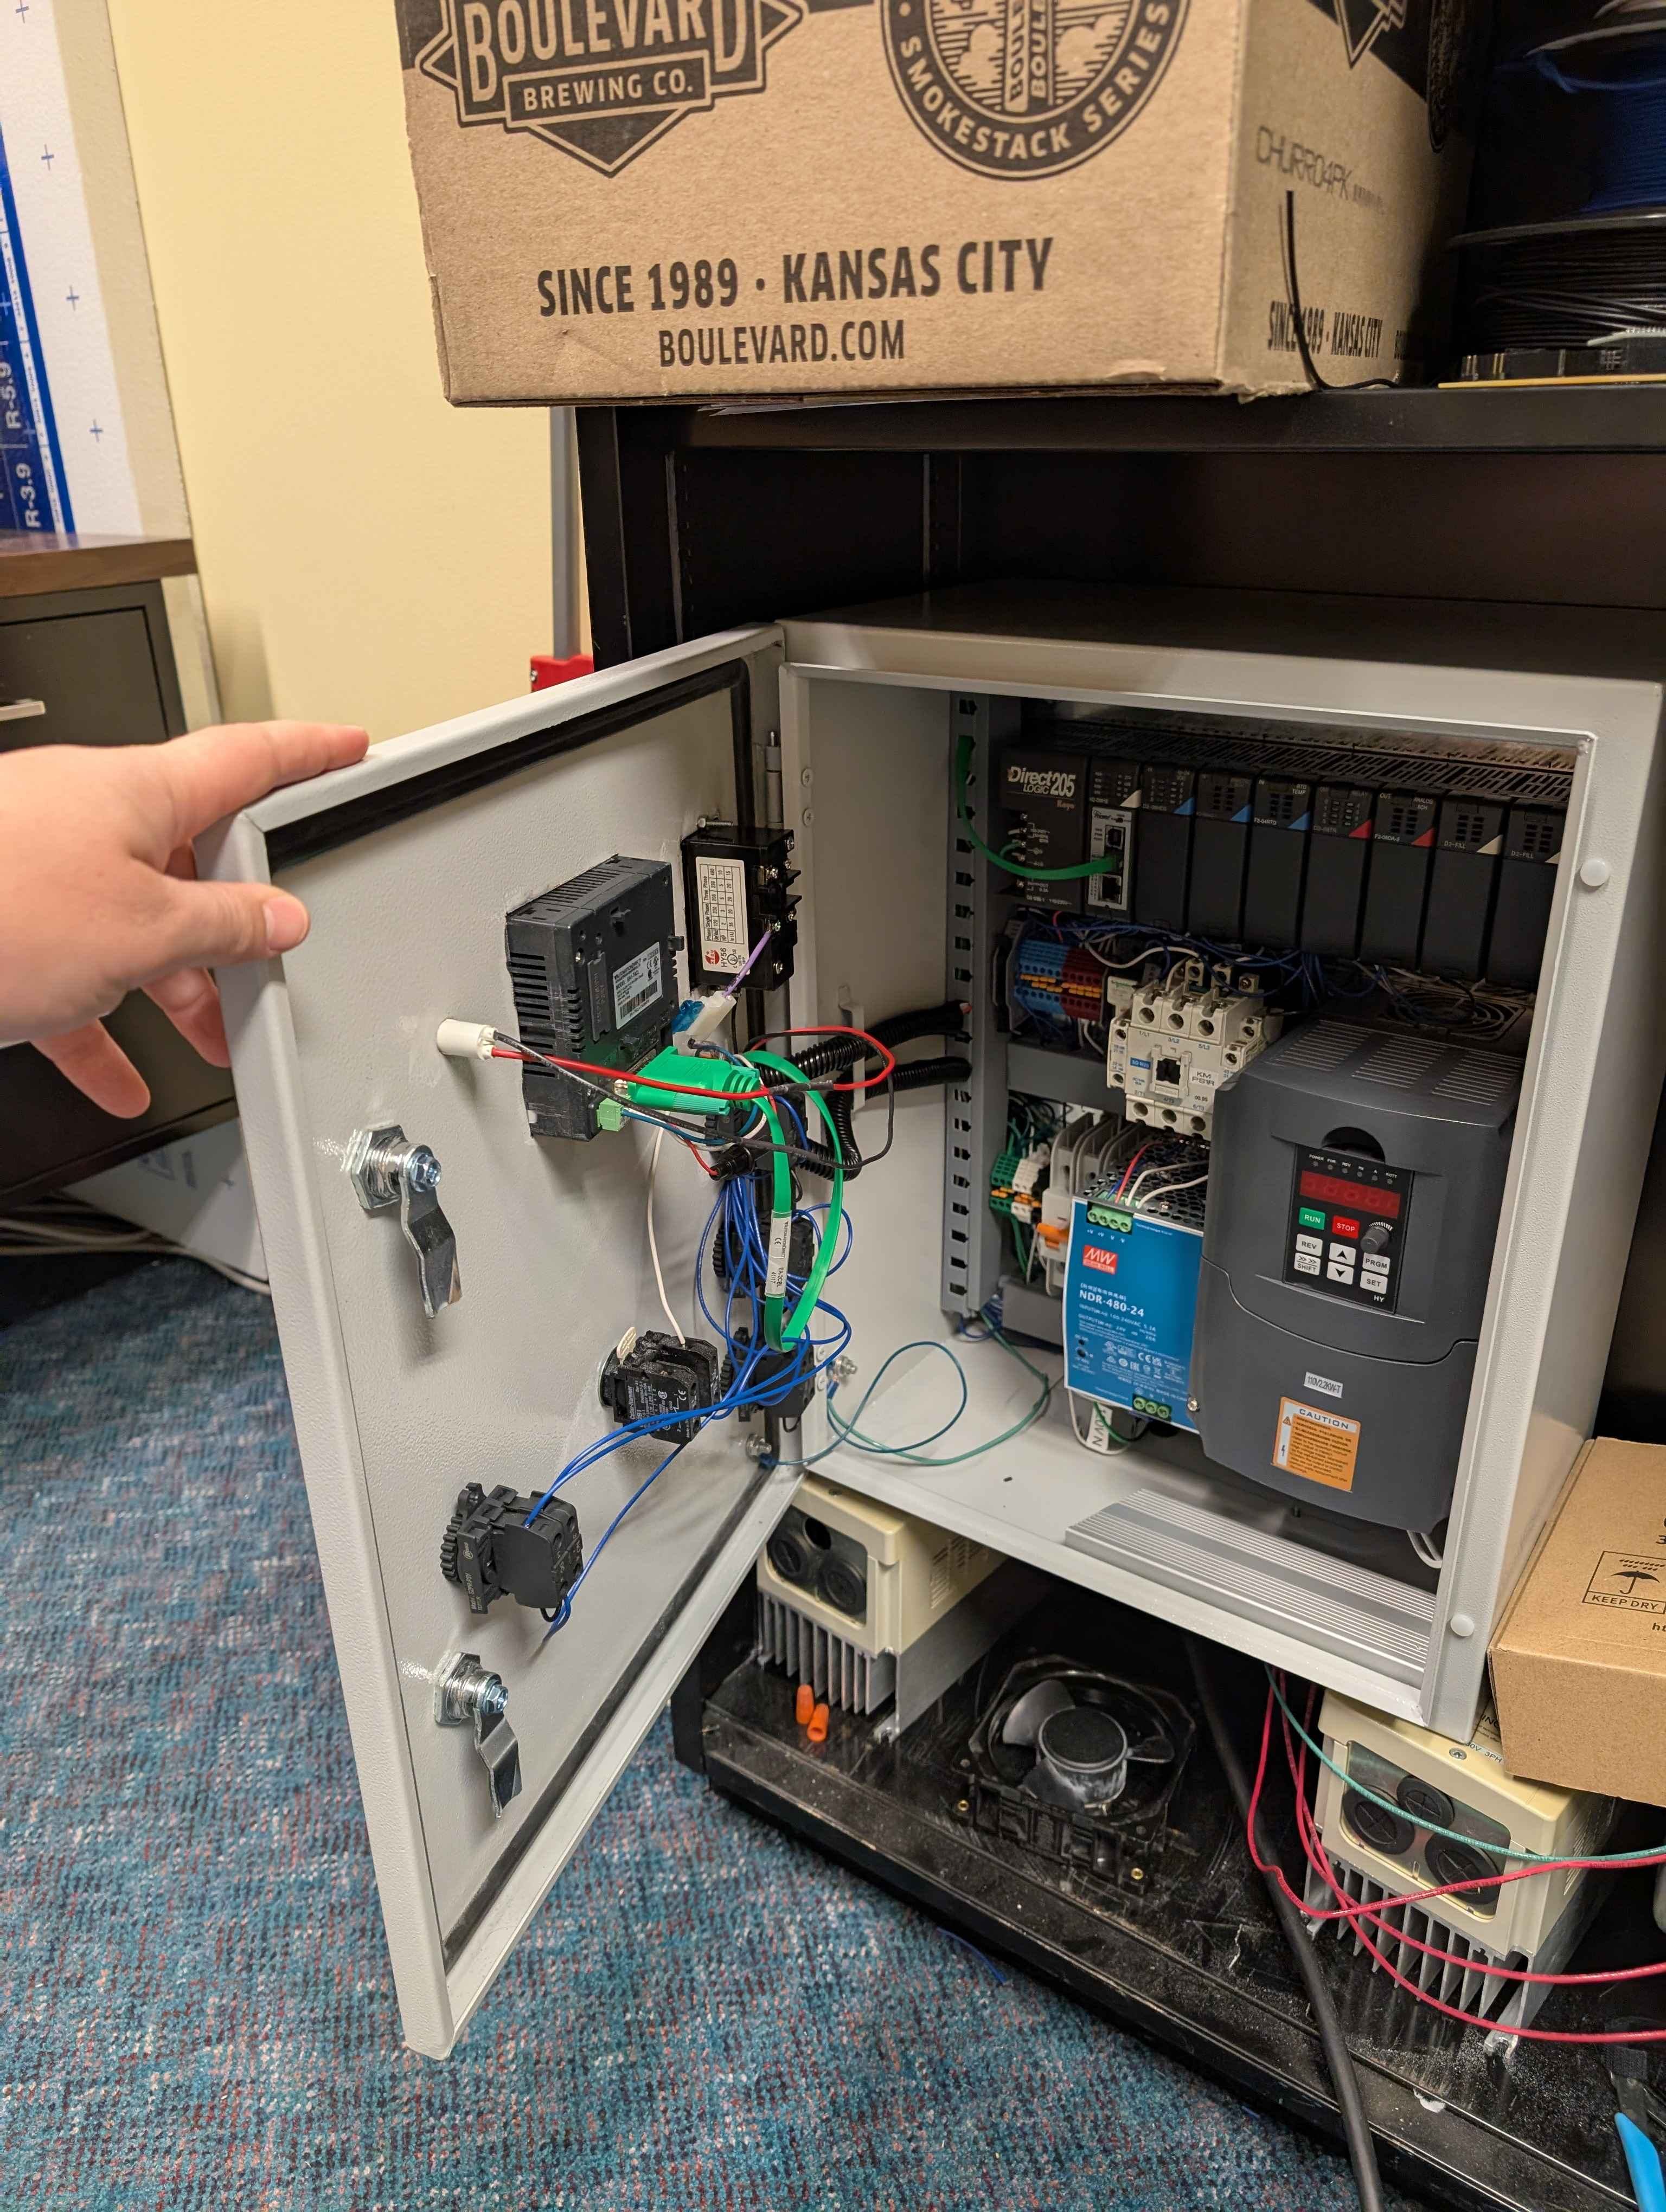
\includegraphics[height=6.5in]{./Pictures/Photo_Inside_Panel.jpg}\hspace{3pt}%
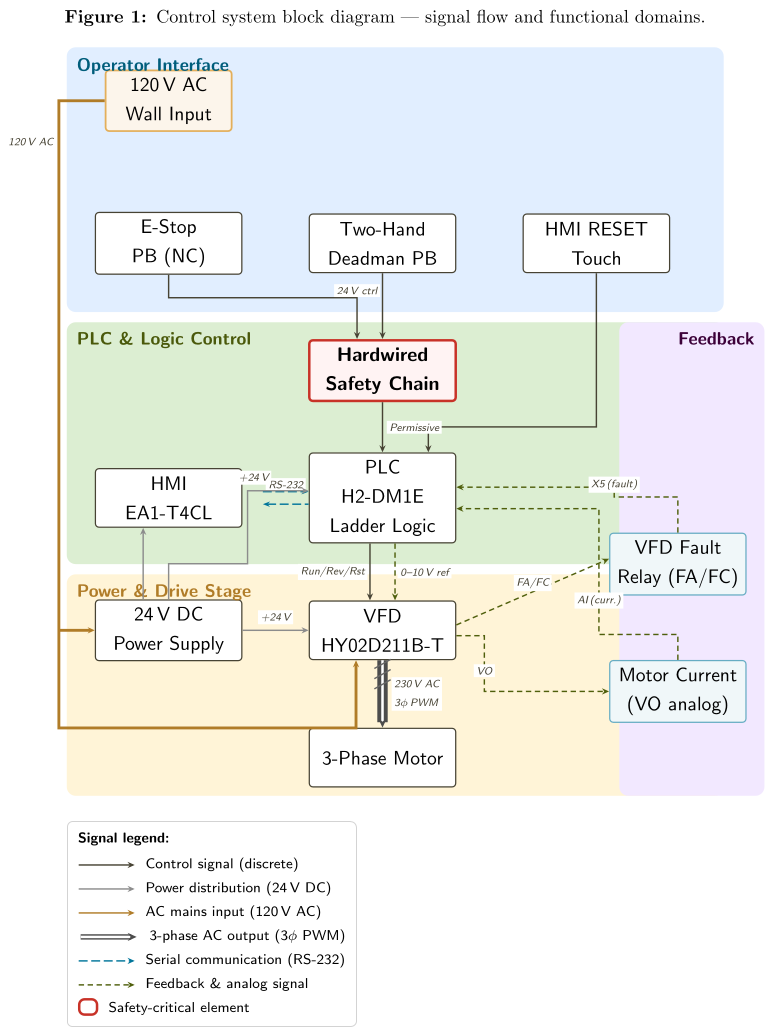
\includegraphics[height=6.5in]{./Pictures/Block_Diagram.png}\\[3pt]
{\small\itshape Operator face \textbullet\ panel interior \textbullet\ system block diagram.}
\end{center}

\columnbreak
%================ COLUMN 2 ================
\postersec{PLC Control}
\begin{itemize}\setlength{\itemsep}{2pt}
  \item \textbf{CPU:} DirectLOGIC 205 + H2-DM1E.
  \item \textbf{I/O:} 8 DC in, 8 relay out, 8 analog in, 4 RTD in, 0--10\,V analog out to the VFD.
  \item \textbf{Program:} 31 rungs in Do-more. Deterministic state machine, 3-strike jam recovery, hard-lockout path.
\end{itemize}

\postersec{HMI}
\begin{itemize}\setlength{\itemsep}{2pt}
  \item \textbf{Panel:} EA1-T4CL C-more Micro-Graphic, 4\,in.~touch.
  \item \textbf{Project:} 4 screens, 27 PLC tags, serial to the CPU.
\end{itemize}

\begin{center}
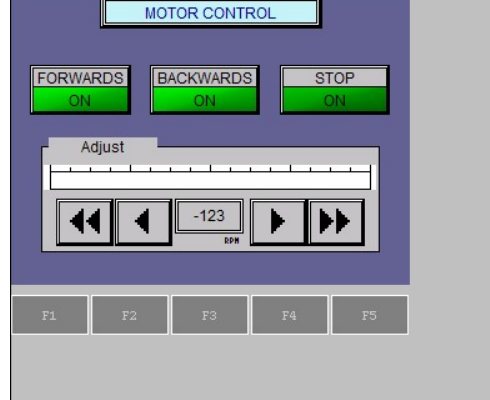
\includegraphics[width=0.235\columnwidth]{./Pictures/HMI_Motor_Control.png}\hspace{2pt}%
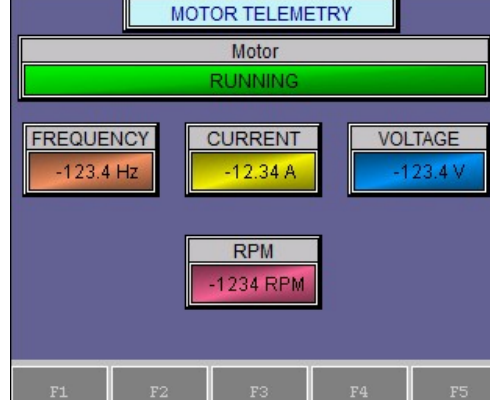
\includegraphics[width=0.235\columnwidth]{./Pictures/HMI_Telemetry.png}\hspace{2pt}%
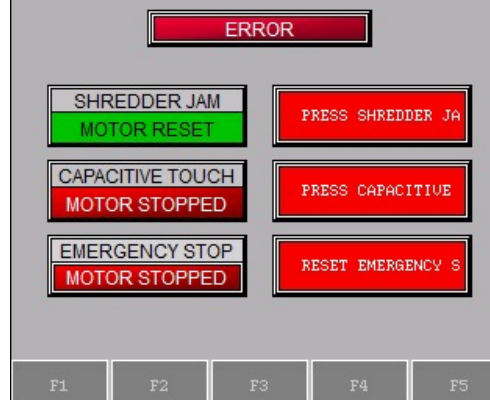
\includegraphics[width=0.235\columnwidth]{./Pictures/HMI_Error.png}\hspace{2pt}%
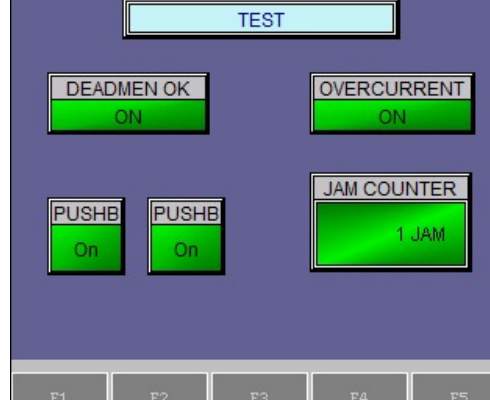
\includegraphics[width=0.235\columnwidth]{./Pictures/HMI_Test.png}\\[2pt]
{\small\itshape Motor Control \textbullet\ Motor Telemetry \textbullet\ Error / Alarm \textbullet\ Test.}
\end{center}

\postersec{Capacitive-Touch Safety (CTSI) Module}
\begin{itemize}\setlength{\itemsep}{2pt}
  \item \textbf{What:} contact-free operator-presence sensor, in-house build.
  \item \textbf{How:} ESP32 reads electrode $\rightarrow$ optocoupler closes 24\,V on PLC \texttt{X7}.
  \item \textbf{Power:} panel 24\,VDC $\rightarrow$ LM2596 buck $\rightarrow$ 3.3\,V to ESP32.
\end{itemize}

\begin{center}
\IfFileExists{./Pictures/Photo_CTSI_Module.jpg}{%
  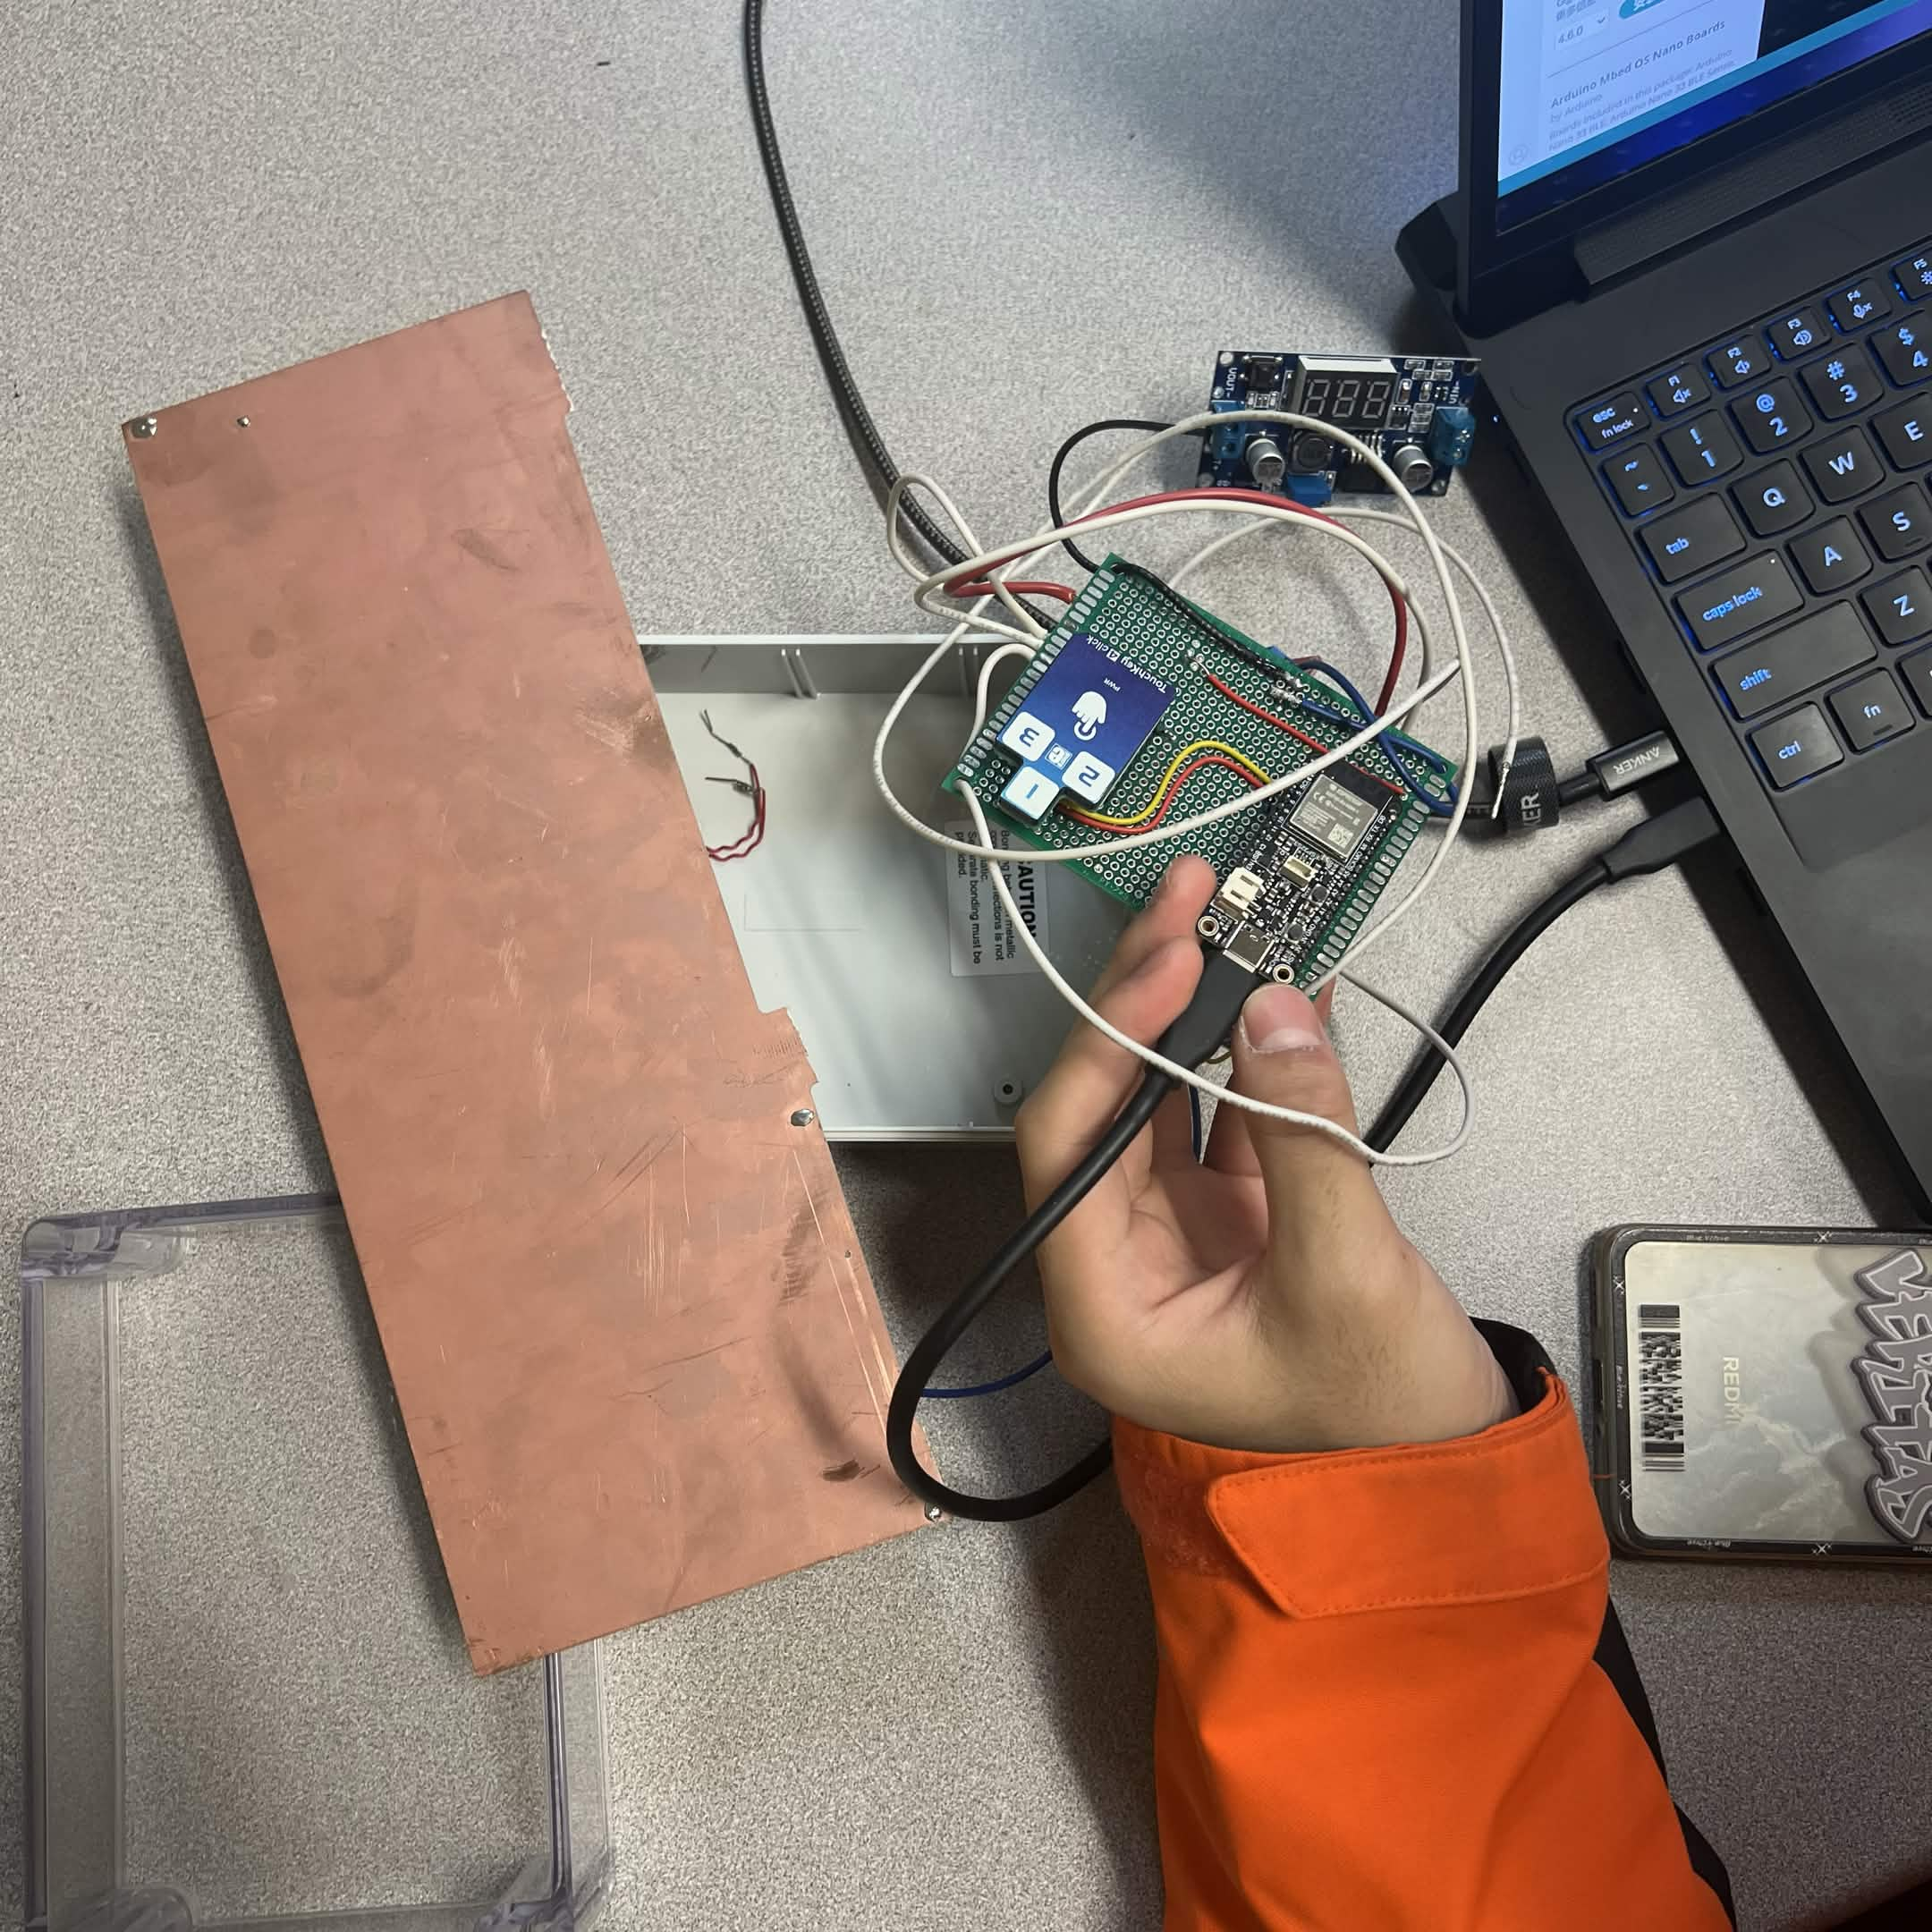
\includegraphics[height=4in]{./Pictures/Photo_CTSI_Module.jpg}%
}{\IfFileExists{./Pictures/Photo_CTSI_Module.png}{%
  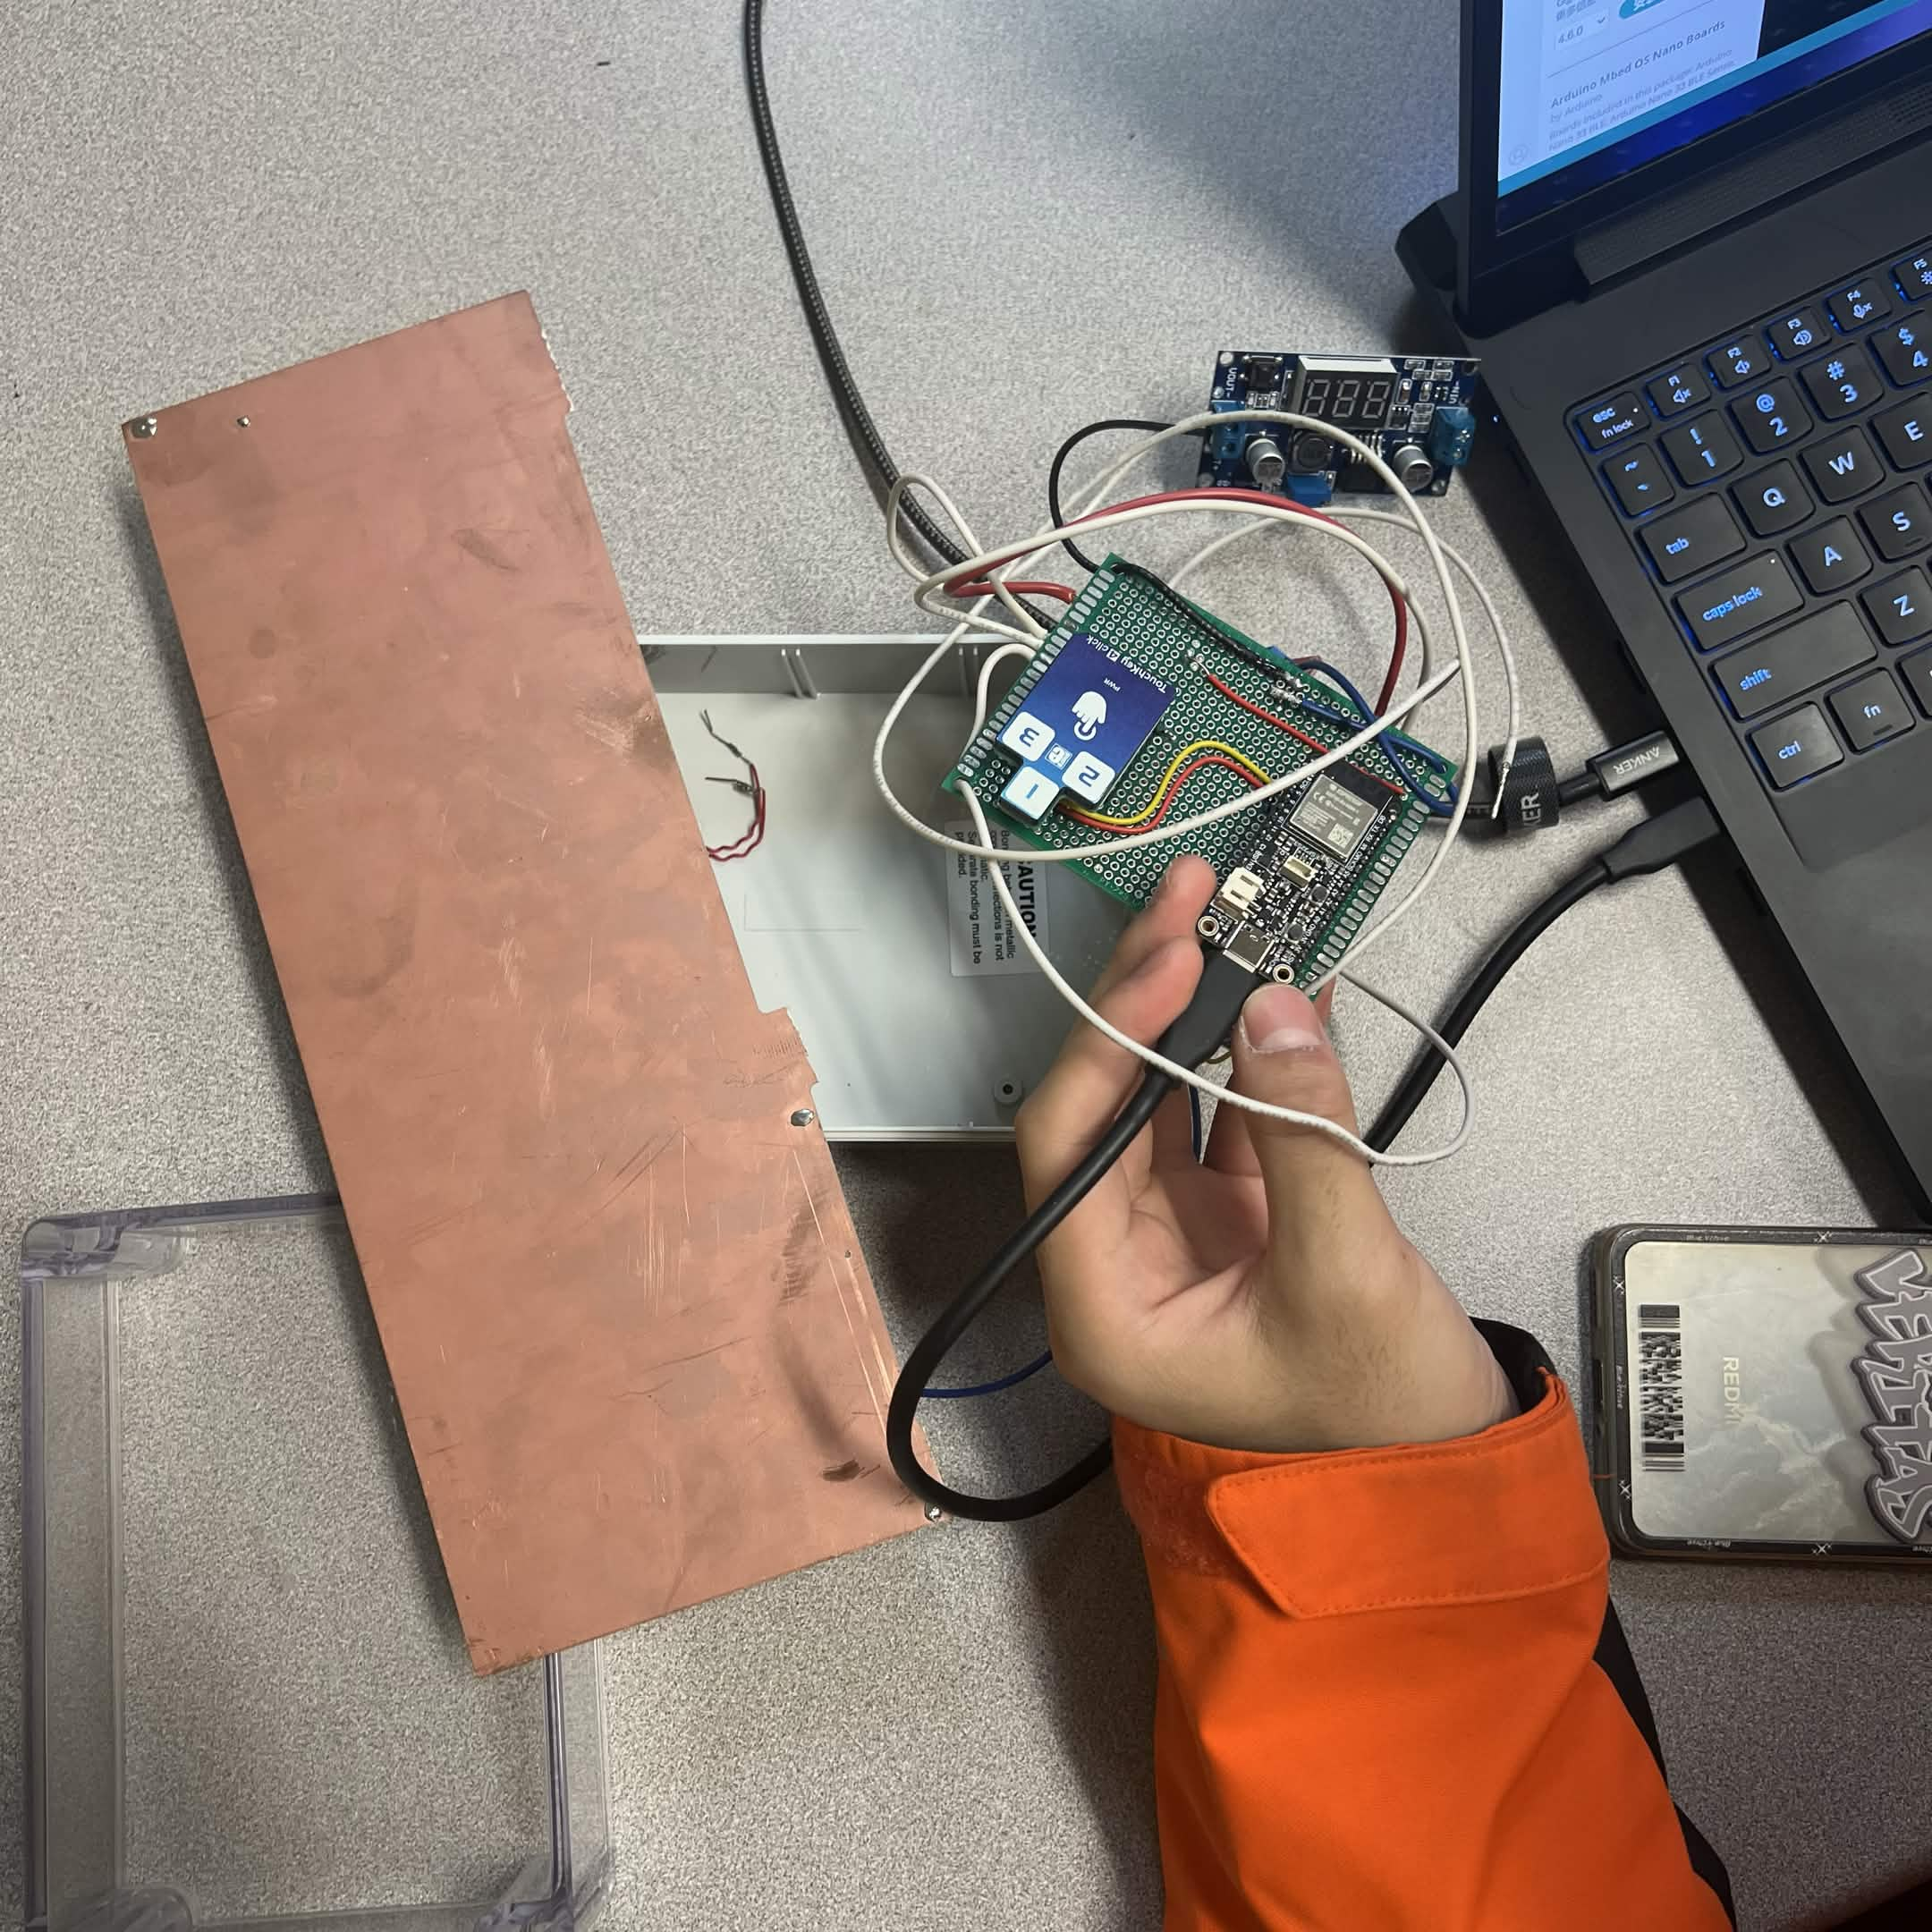
\includegraphics[height=4in]{./Pictures/Photo_CTSI_Module.png}%
}{%
  \fbox{\begin{minipage}[c][1.6in][c]{0.95\columnwidth}\centering
    \sffamily\color{PSUgray}\itshape
    \textbf{[ CTSI module photo ]}\\[4pt]
    Drop \texttt{Photo\_CTSI\_Module.jpg} into\\
    \texttt{src/Pictures/} to insert it here.
  \end{minipage}}%
}}\\[2pt]
{\small\itshape ESP32 + LM2596 buck + optocoupler module wired to PLC \texttt{X7}.}
\end{center}

\textbf{On touch (rung 28):} motor stops, fault LED on, HMI jumps to
ERROR -- independent of the deadman / E-stop chain.

\textbf{Status:} bench-validated. Full-machine test pending the
ME prototype.

\columnbreak
%================ COLUMN 3 ================
\postersec{Panel CAD Layout}
\begin{center}
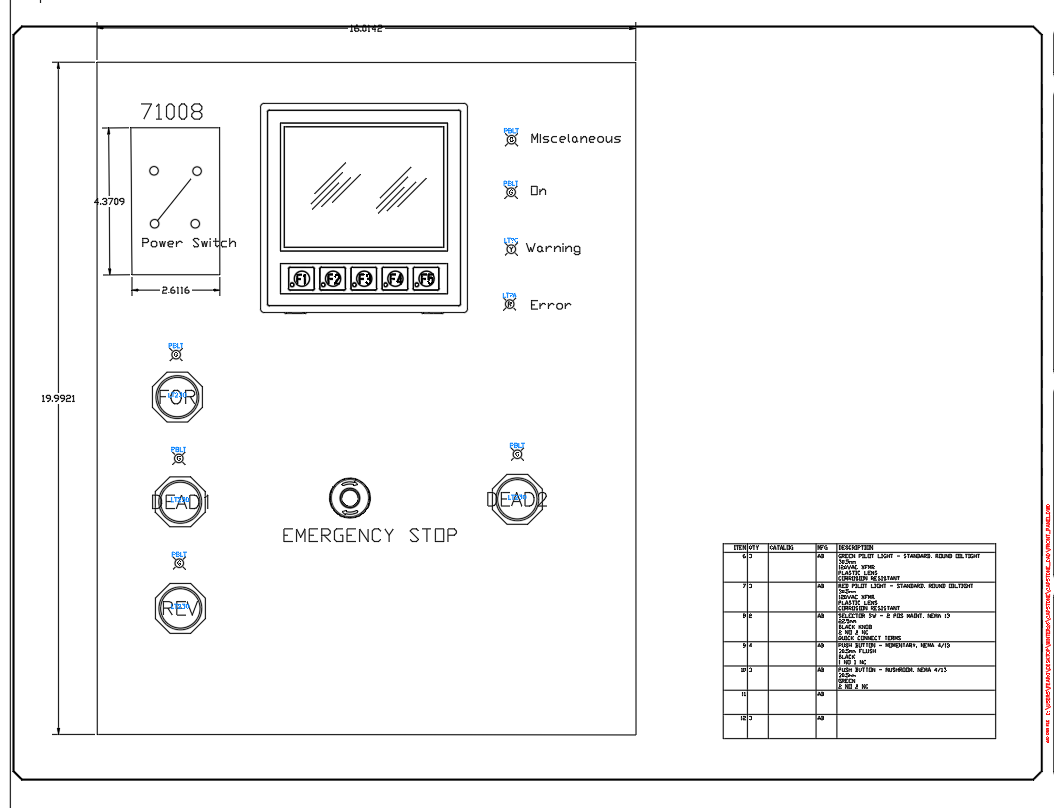
\includegraphics[height=3.8in]{./Pictures/Front_Panel_CAD.png}\hspace{4pt}%
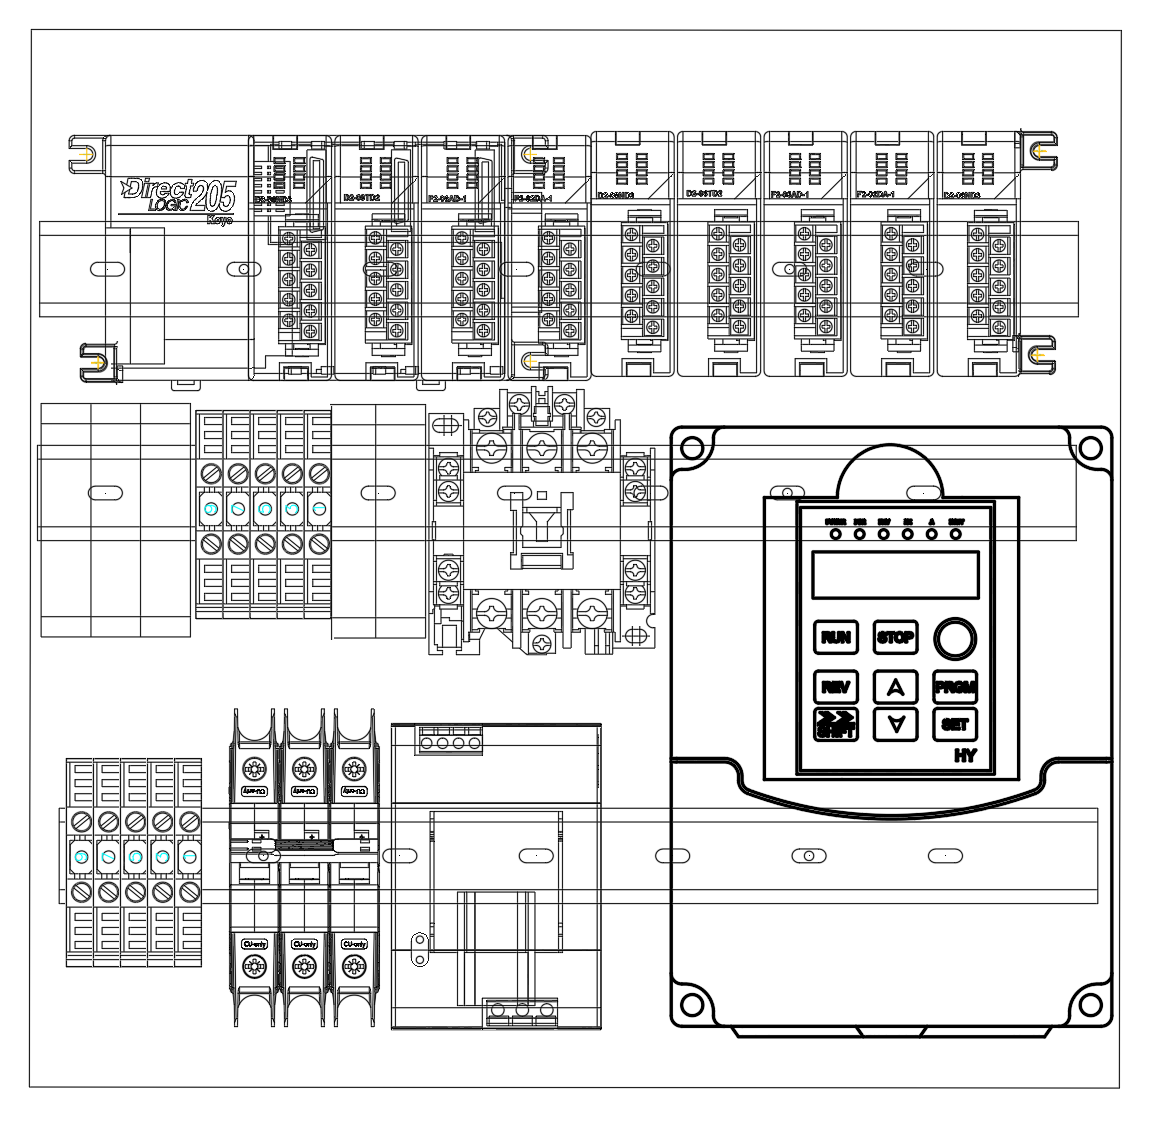
\includegraphics[height=3.8in]{./Pictures/Panel_CAD_Layout.png}\\[2pt]
{\small\itshape AutoCAD Electrical: front operator face (left) \textbullet\ back-plate component layout (right).}
\end{center}

\postersec{Safety \& Compliance}
\begin{itemize}\setlength{\itemsep}{2pt}
  \item \textbf{E-stop:} Category 0 stop. Eaton E22B1 NC mushroom in series with the SD-N35 contactor coil. Drops the contactor independently of the PLC.
  \item \textbf{Two-hand / deadman:} both pushbuttons must be held to enable the motor (PLC X2 AND X3).
  \item \textbf{Overcurrent / jam:} VFD over-torque trip (\texttt{PD124 = 150\%}, \texttt{PD125 = 3\,s}) on PLC X5; ladder runs the 3-strike unjam routine.
  \item \textbf{Enclosure:} Vorksmen SEB001 steel, NEMA Type 12.
  \item \textbf{Compliance:} NFPA 70/79, NEMA 250 / ICS / MG~1, ISO 12100, 13849-1 (Cat~B--1 / PL b--c), 13850, 13851, OSHA 1910.147.
\end{itemize}

\postersec{Results}
\textbf{All EE ``Must'' requirements met} -- motor control, NFPA-70
design, E-stop + overload + interlock, HMI, and the \$1{,}000 budget.

\textbf{Constraint:} ME team did not deliver the mechanical
prototype, so full-machine integration testing was not possible.
All EE validation is bench-only.

\textbf{Working:}
\begin{itemize}\setlength{\itemsep}{2pt}
  \item Panel built, wired, bench-validated.
  \item All 31 ladder rungs scan correctly.
  \item All four HMI screens operate; tags match the PLC.
  \item Speed reference verified end to end.
  \item Jam recovery verified: overcurrent $\rightarrow$ 2\,s reverse $\rightarrow$ coast-to-stop.
\end{itemize}
\textbf{Wired, programming pending:}
\begin{itemize}\setlength{\itemsep}{2pt}
  \item \textbf{CTSI:} module destroyed in bring-up. \texttt{X7} input,
        optocoupler, and rung 28 ready for the replacement.
  \item \textbf{Jam counter:} counts in the PLC, not yet on the HMI.
  \item \textbf{V / I telemetry:} analog path wired and scaled, but
        live values unstable. VFD analog-out parameters + PLC scaling
        need a second pass.
\end{itemize}

\end{multicols}

\vspace{8pt}

% ============== FULL-WIDTH LADDER LOGIC STRIP ==============
\noindent
\begin{tcolorbox}[
  enhanced, sharp corners, boxrule=0pt, frame hidden,
  interior style={top color=PSUgreen, bottom color=PSUgreen!90!black},
  coltext=white,
  left=14pt, right=14pt, top=6pt, bottom=6pt,
  width=\textwidth,
  fontupper=\sffamily\bfseries\large,
  drop shadow=PSUgray!40,
]
Complete Ladder Logic --- 31 rungs across 7 pages
\end{tcolorbox}
\vspace{4pt}
\noindent
\begin{minipage}{\textwidth}
\centering
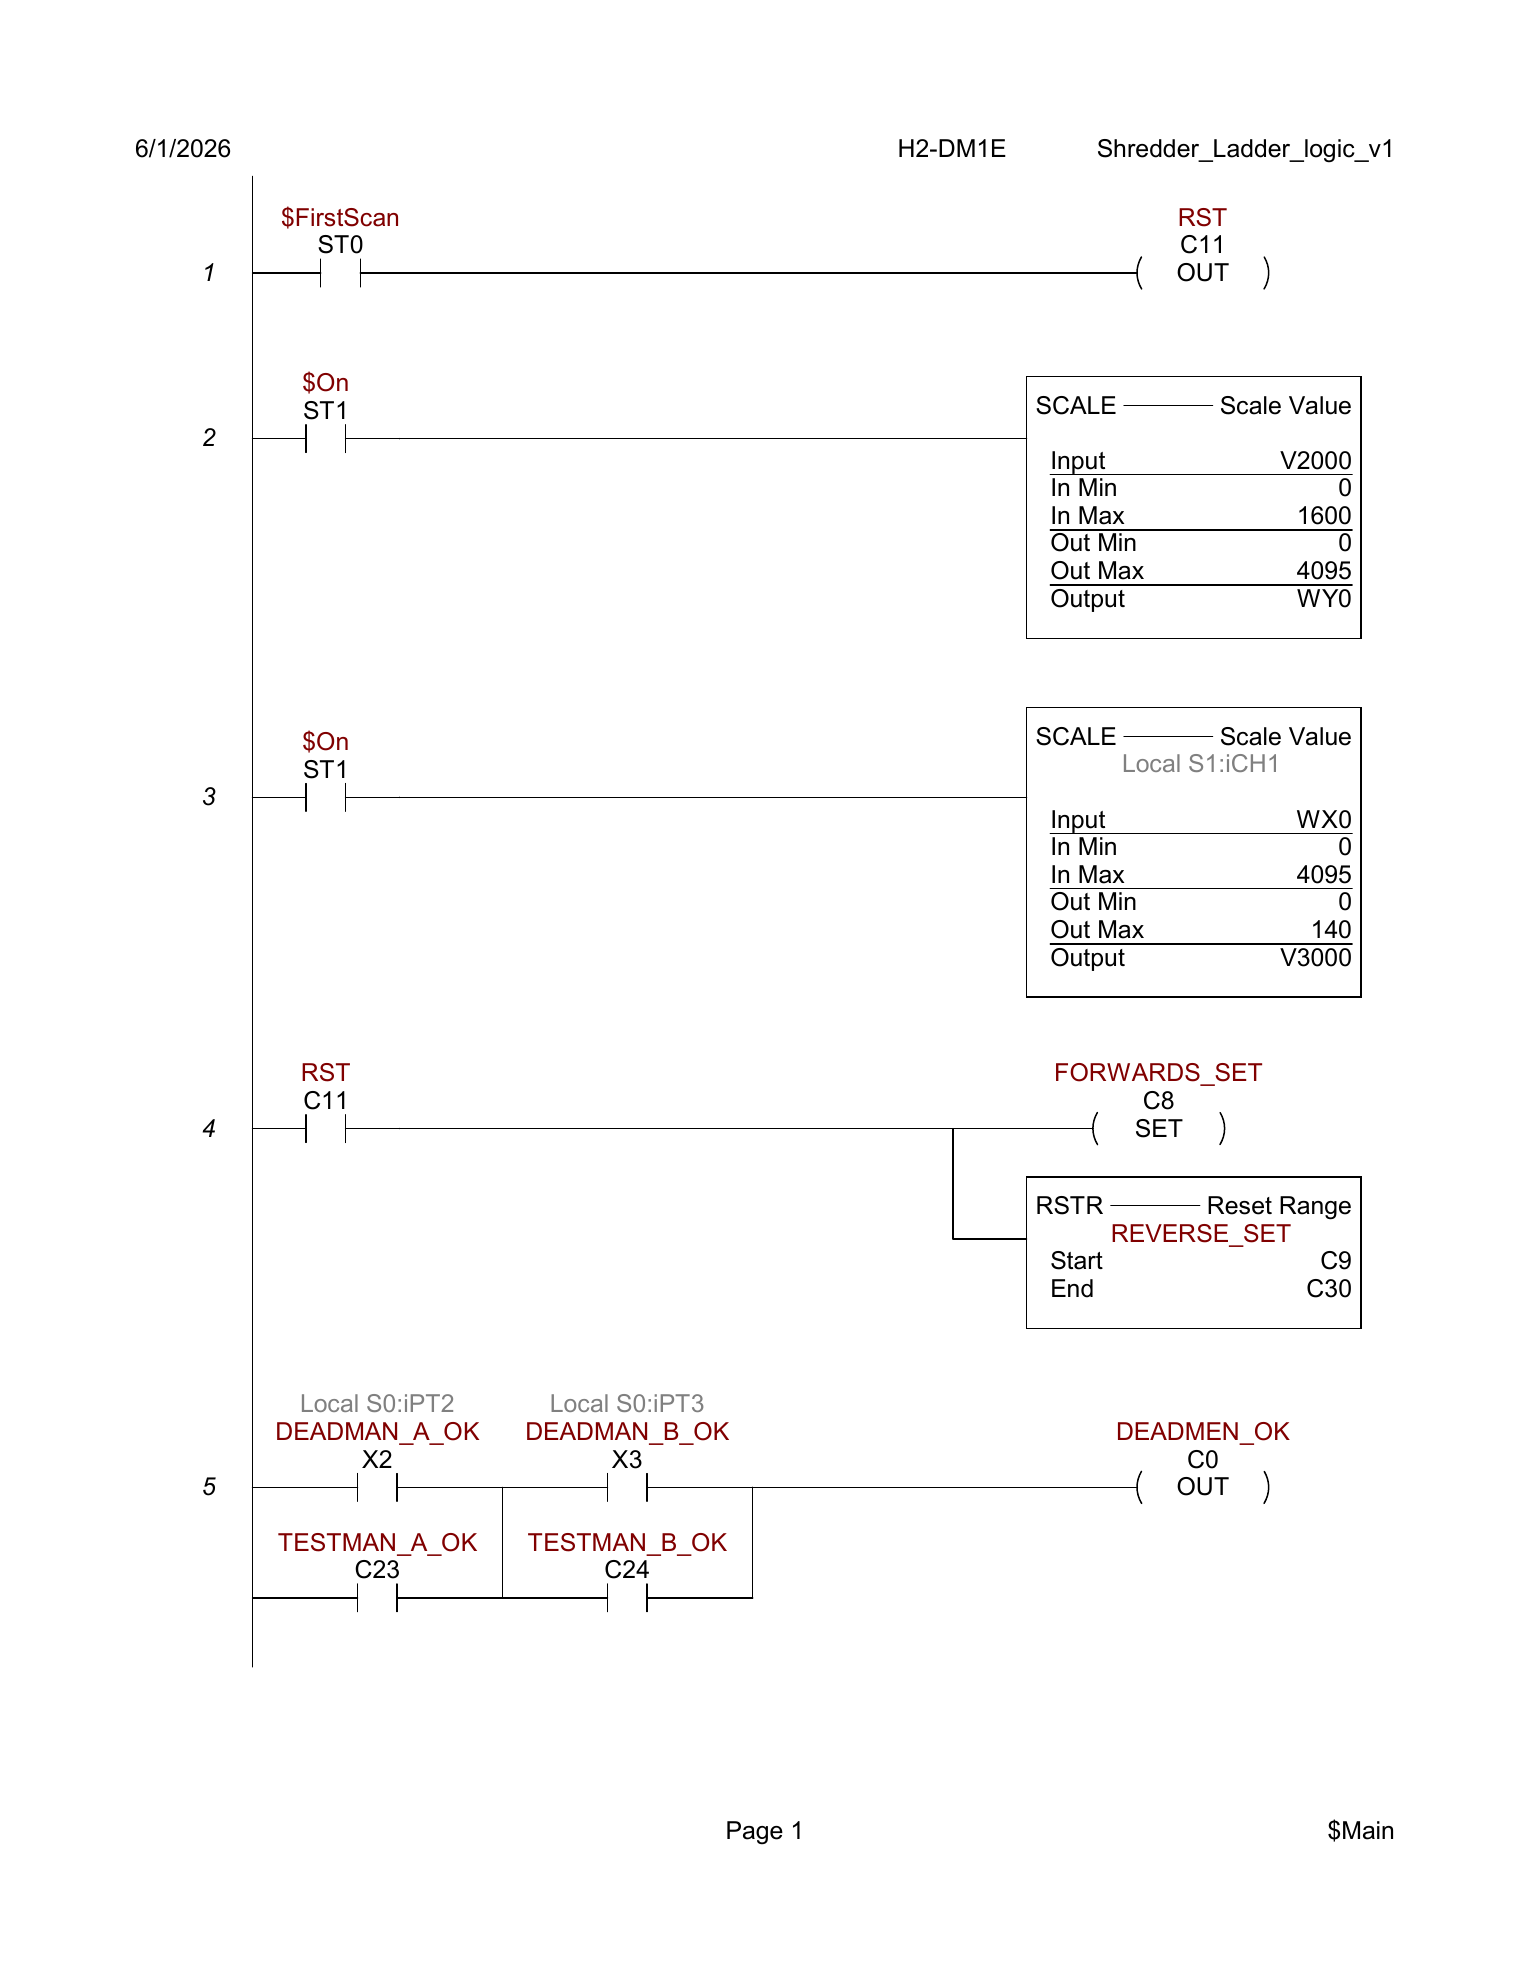
\includegraphics[height=6.5in]{./Pictures/Ladder_1.png}\hspace{3pt}%
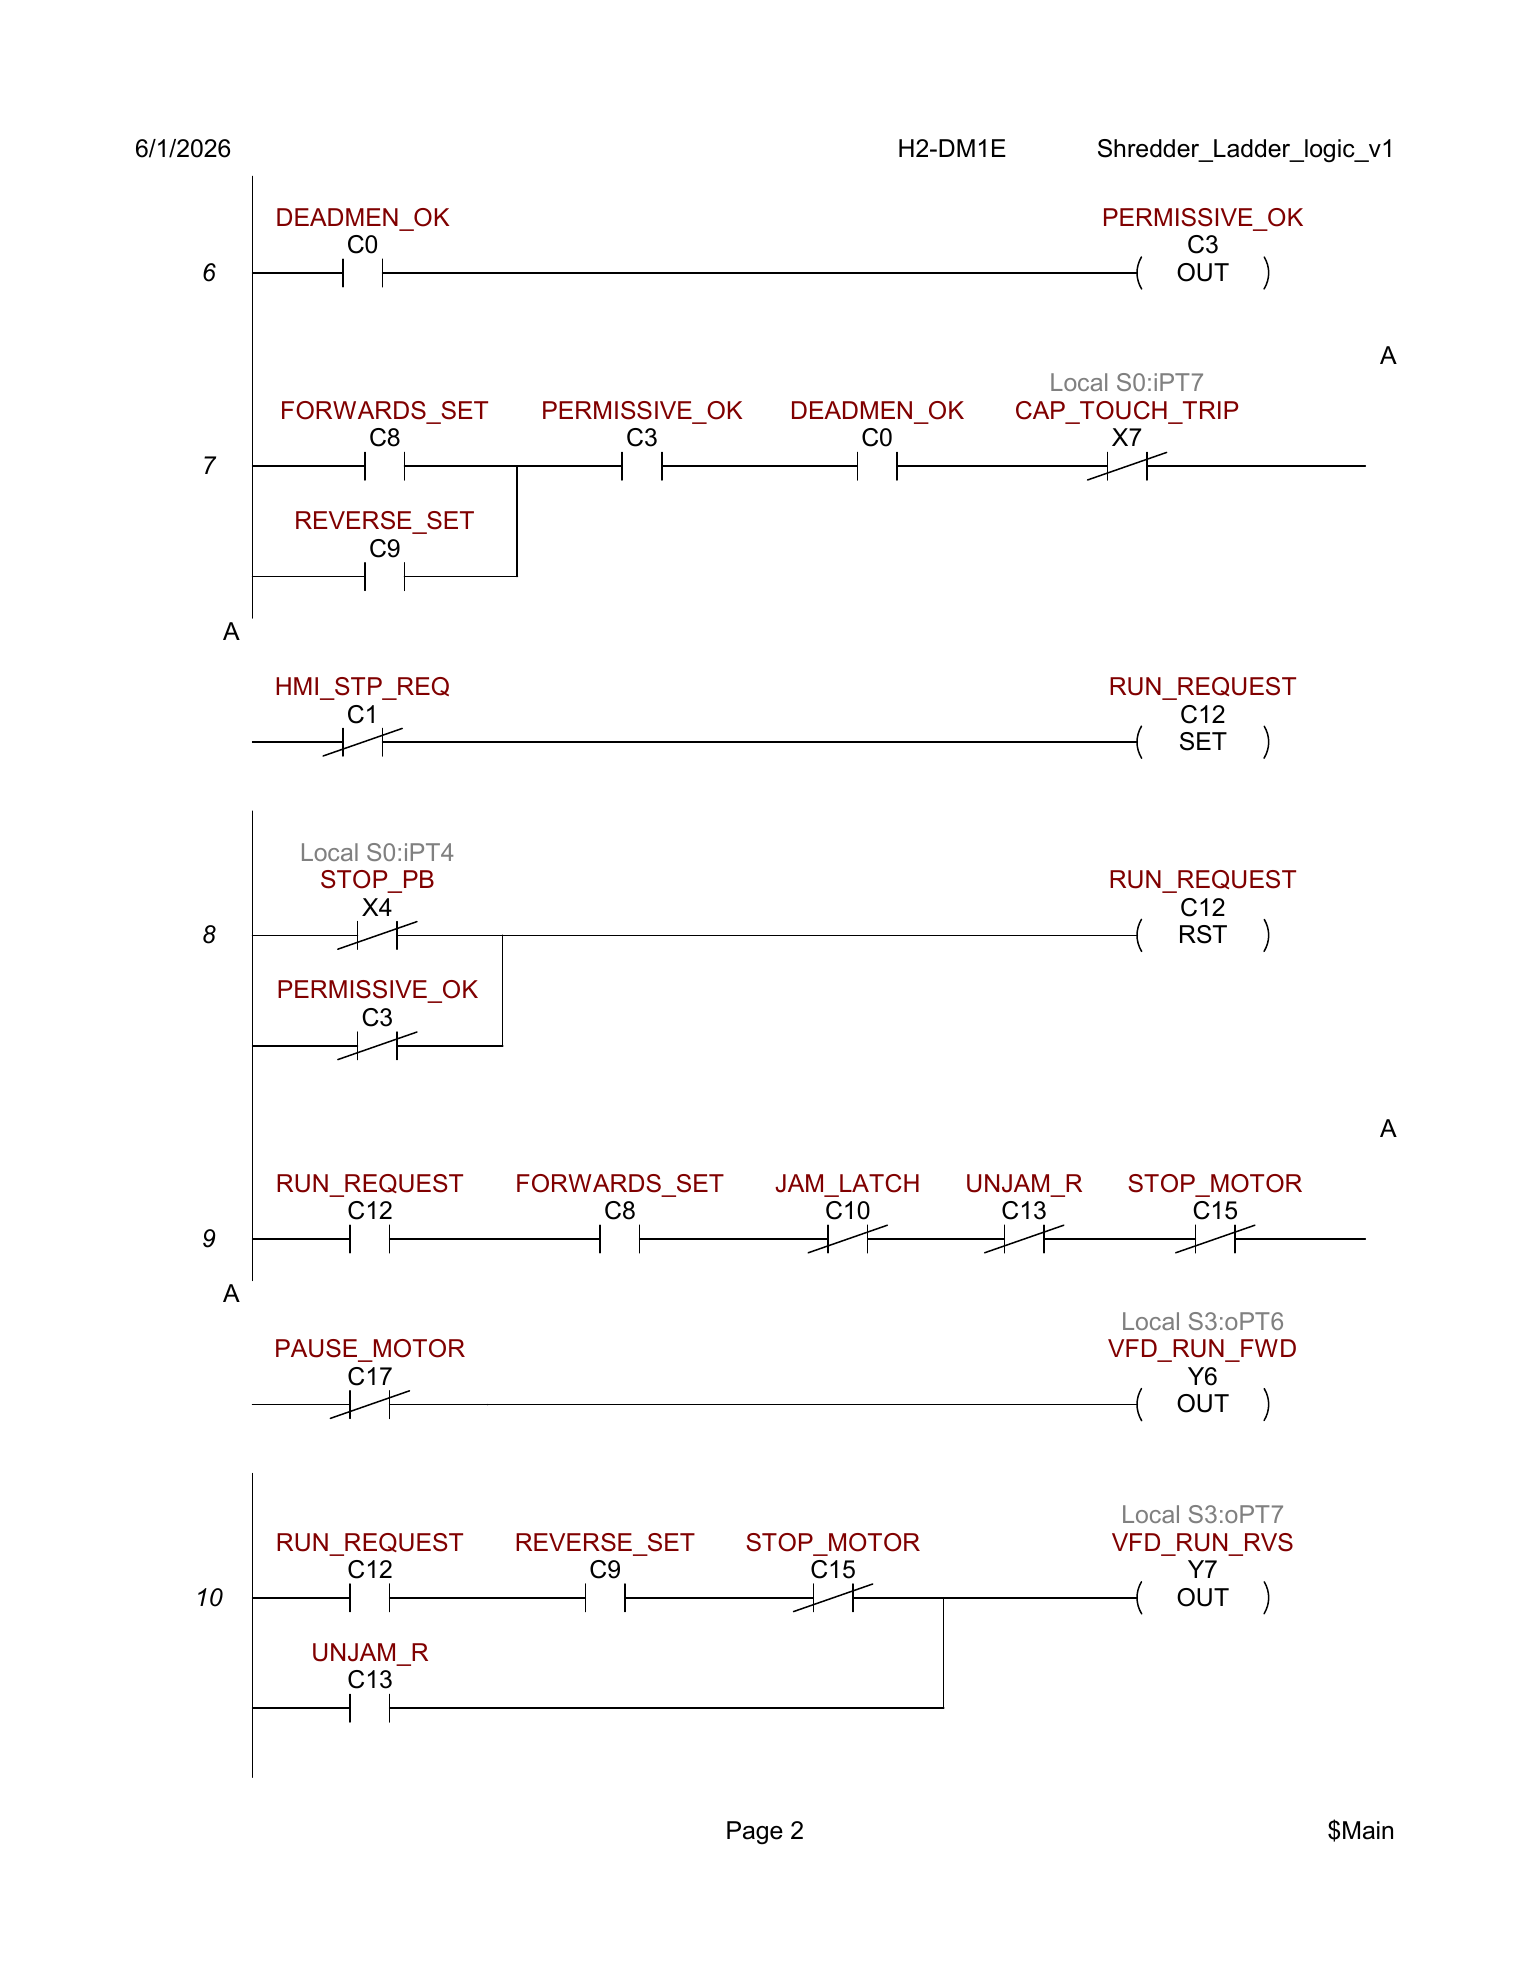
\includegraphics[height=6.5in]{./Pictures/Ladder_2.png}\hspace{3pt}%
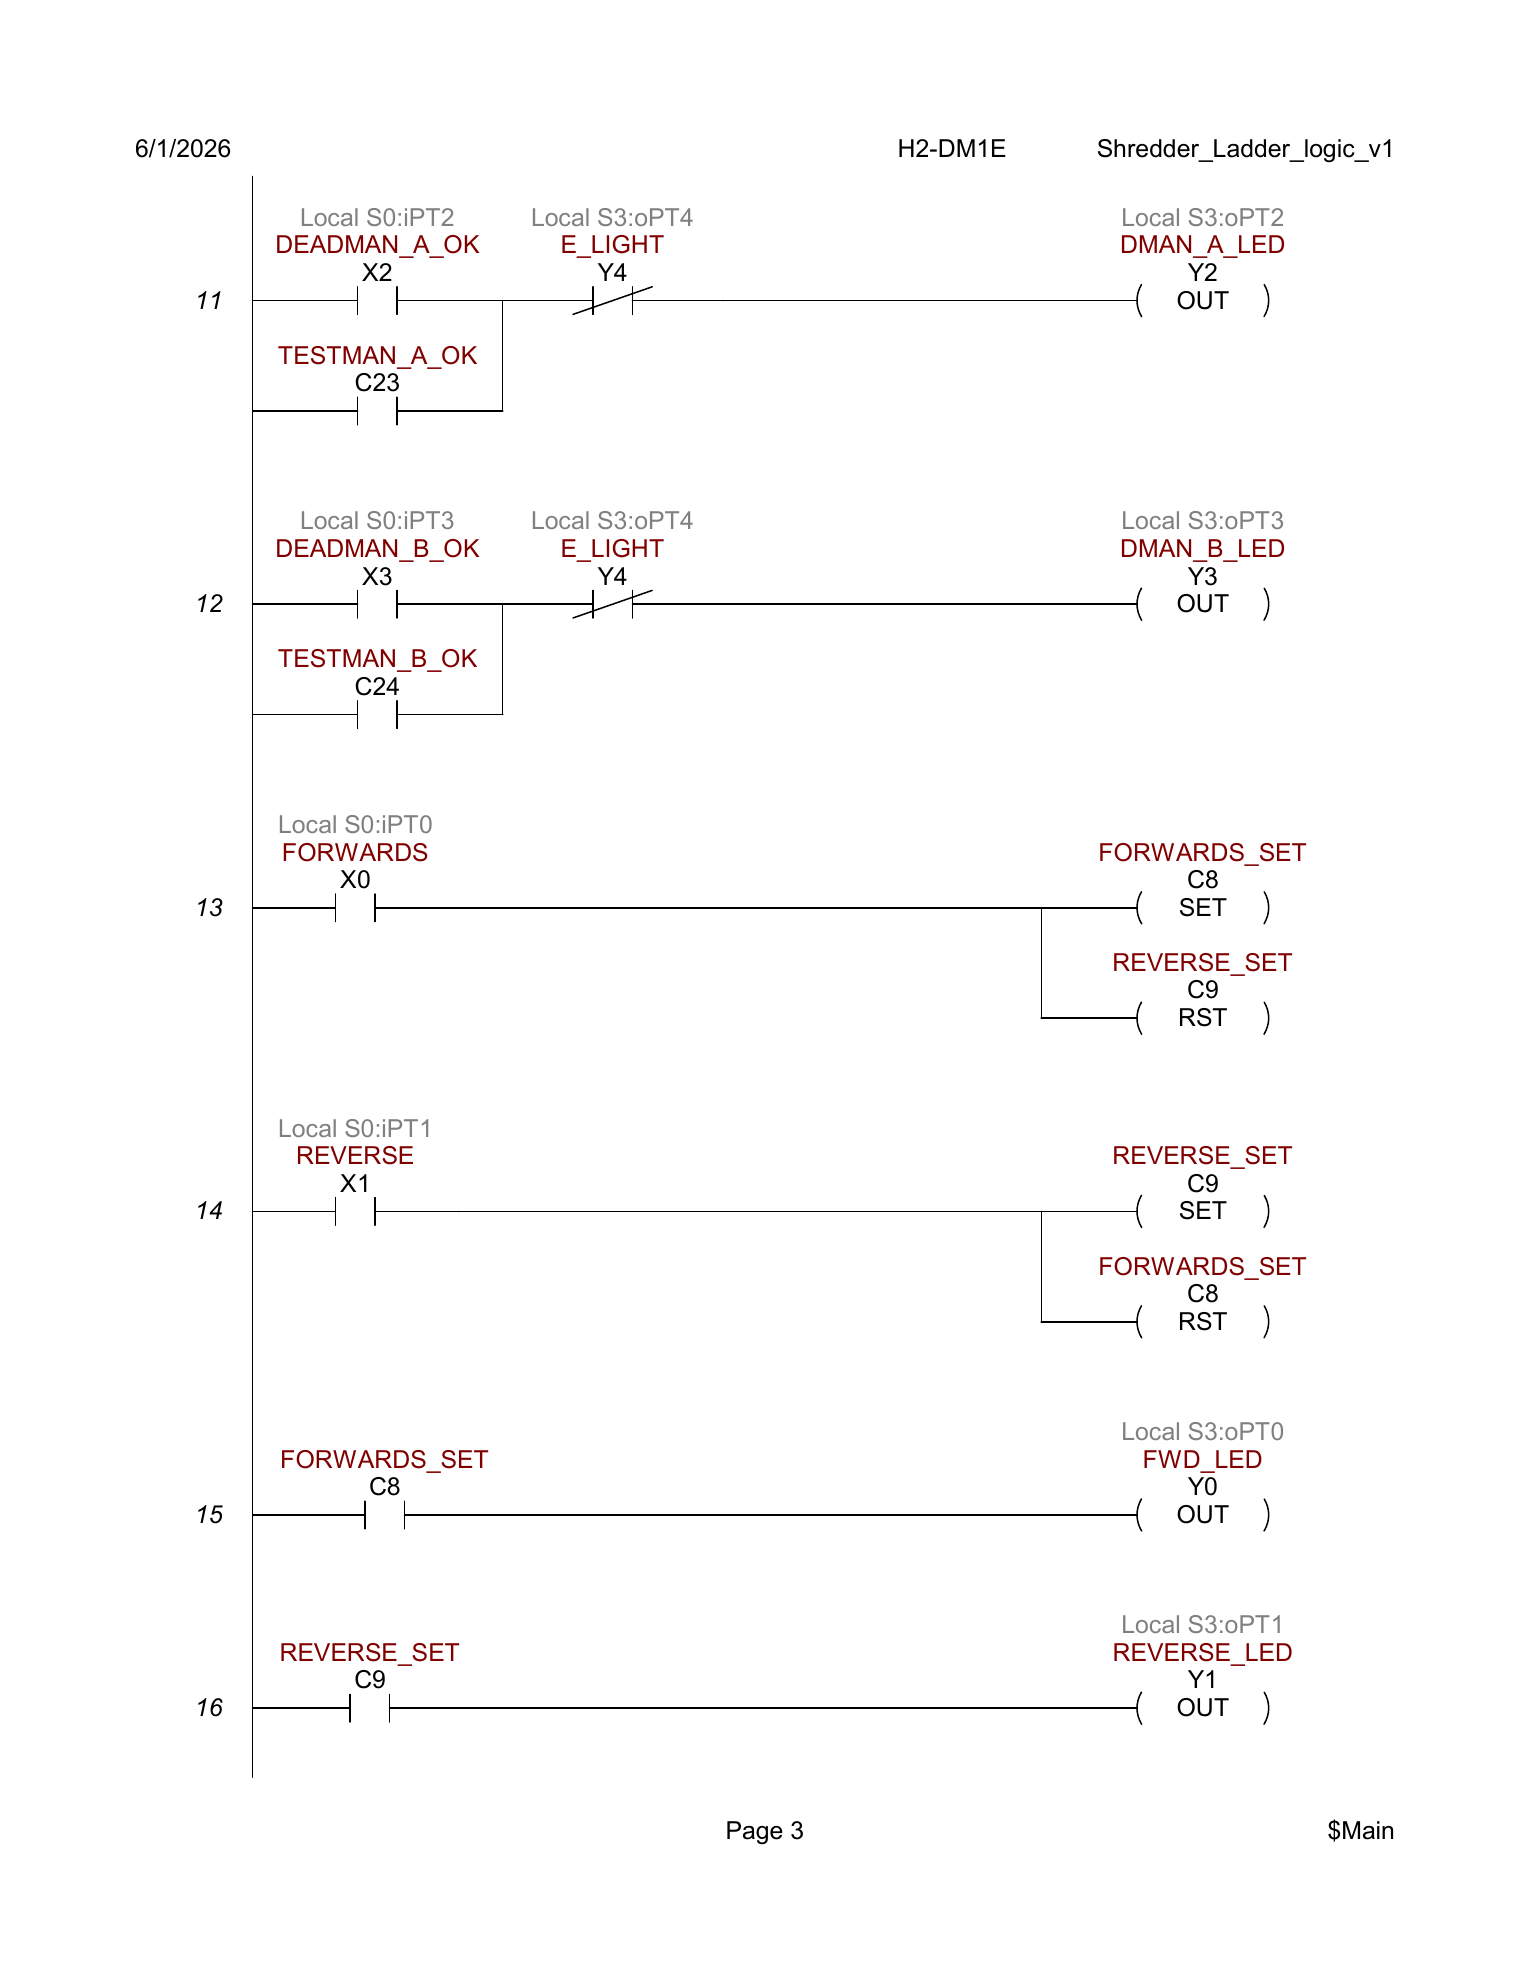
\includegraphics[height=6.5in]{./Pictures/Ladder_3.png}\hspace{3pt}%
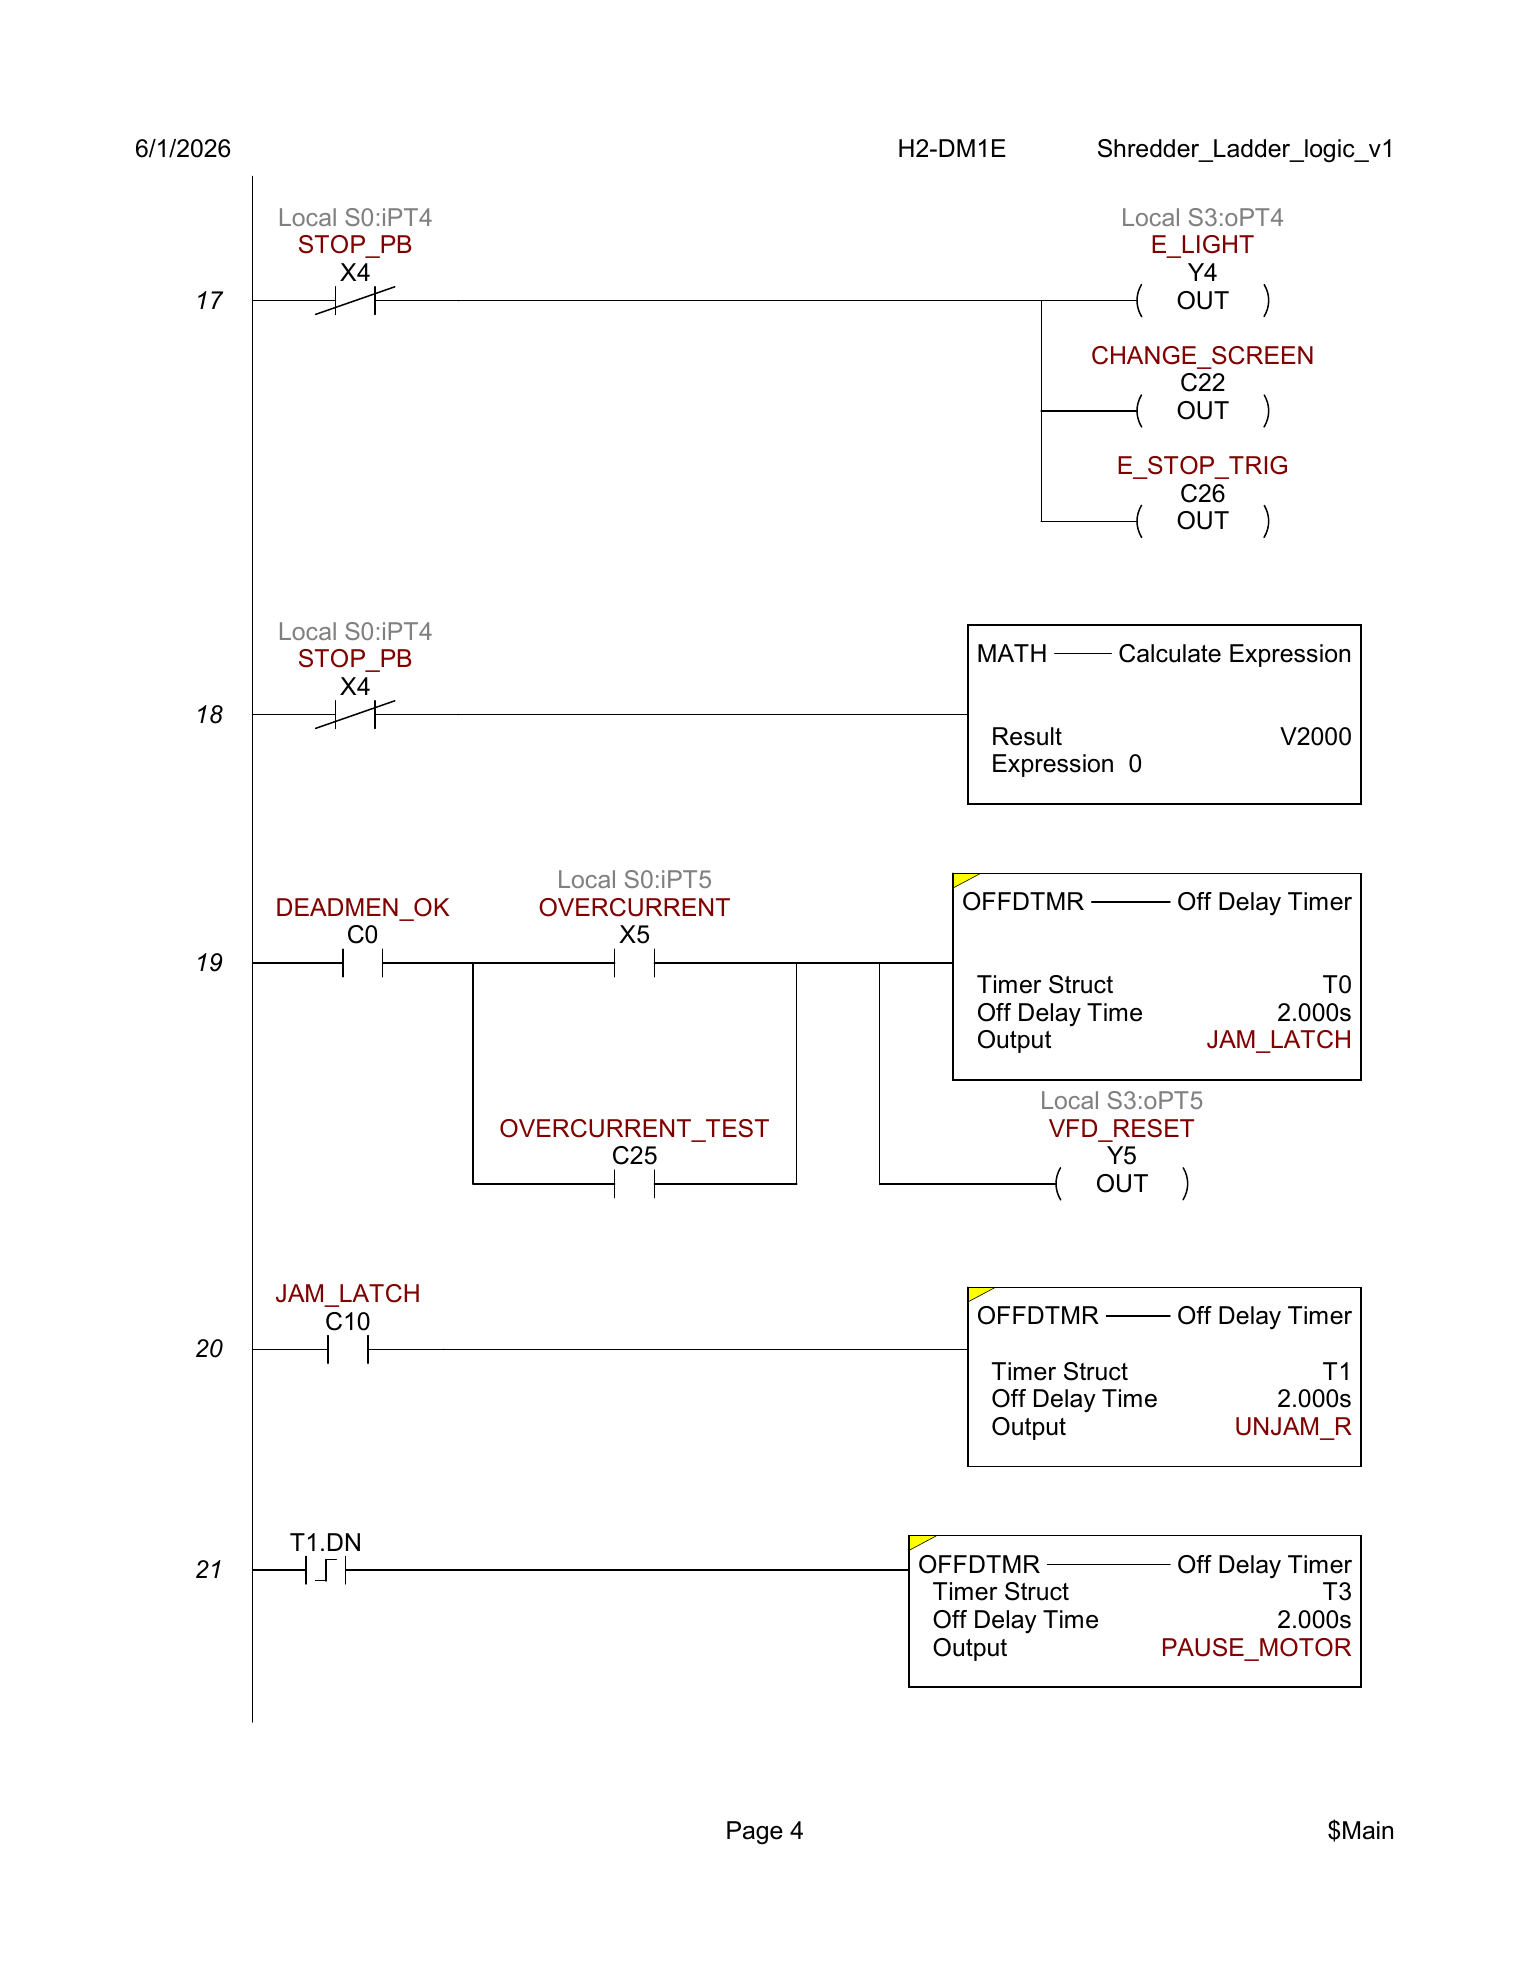
\includegraphics[height=6.5in]{./Pictures/Ladder_4.png}\hspace{3pt}%
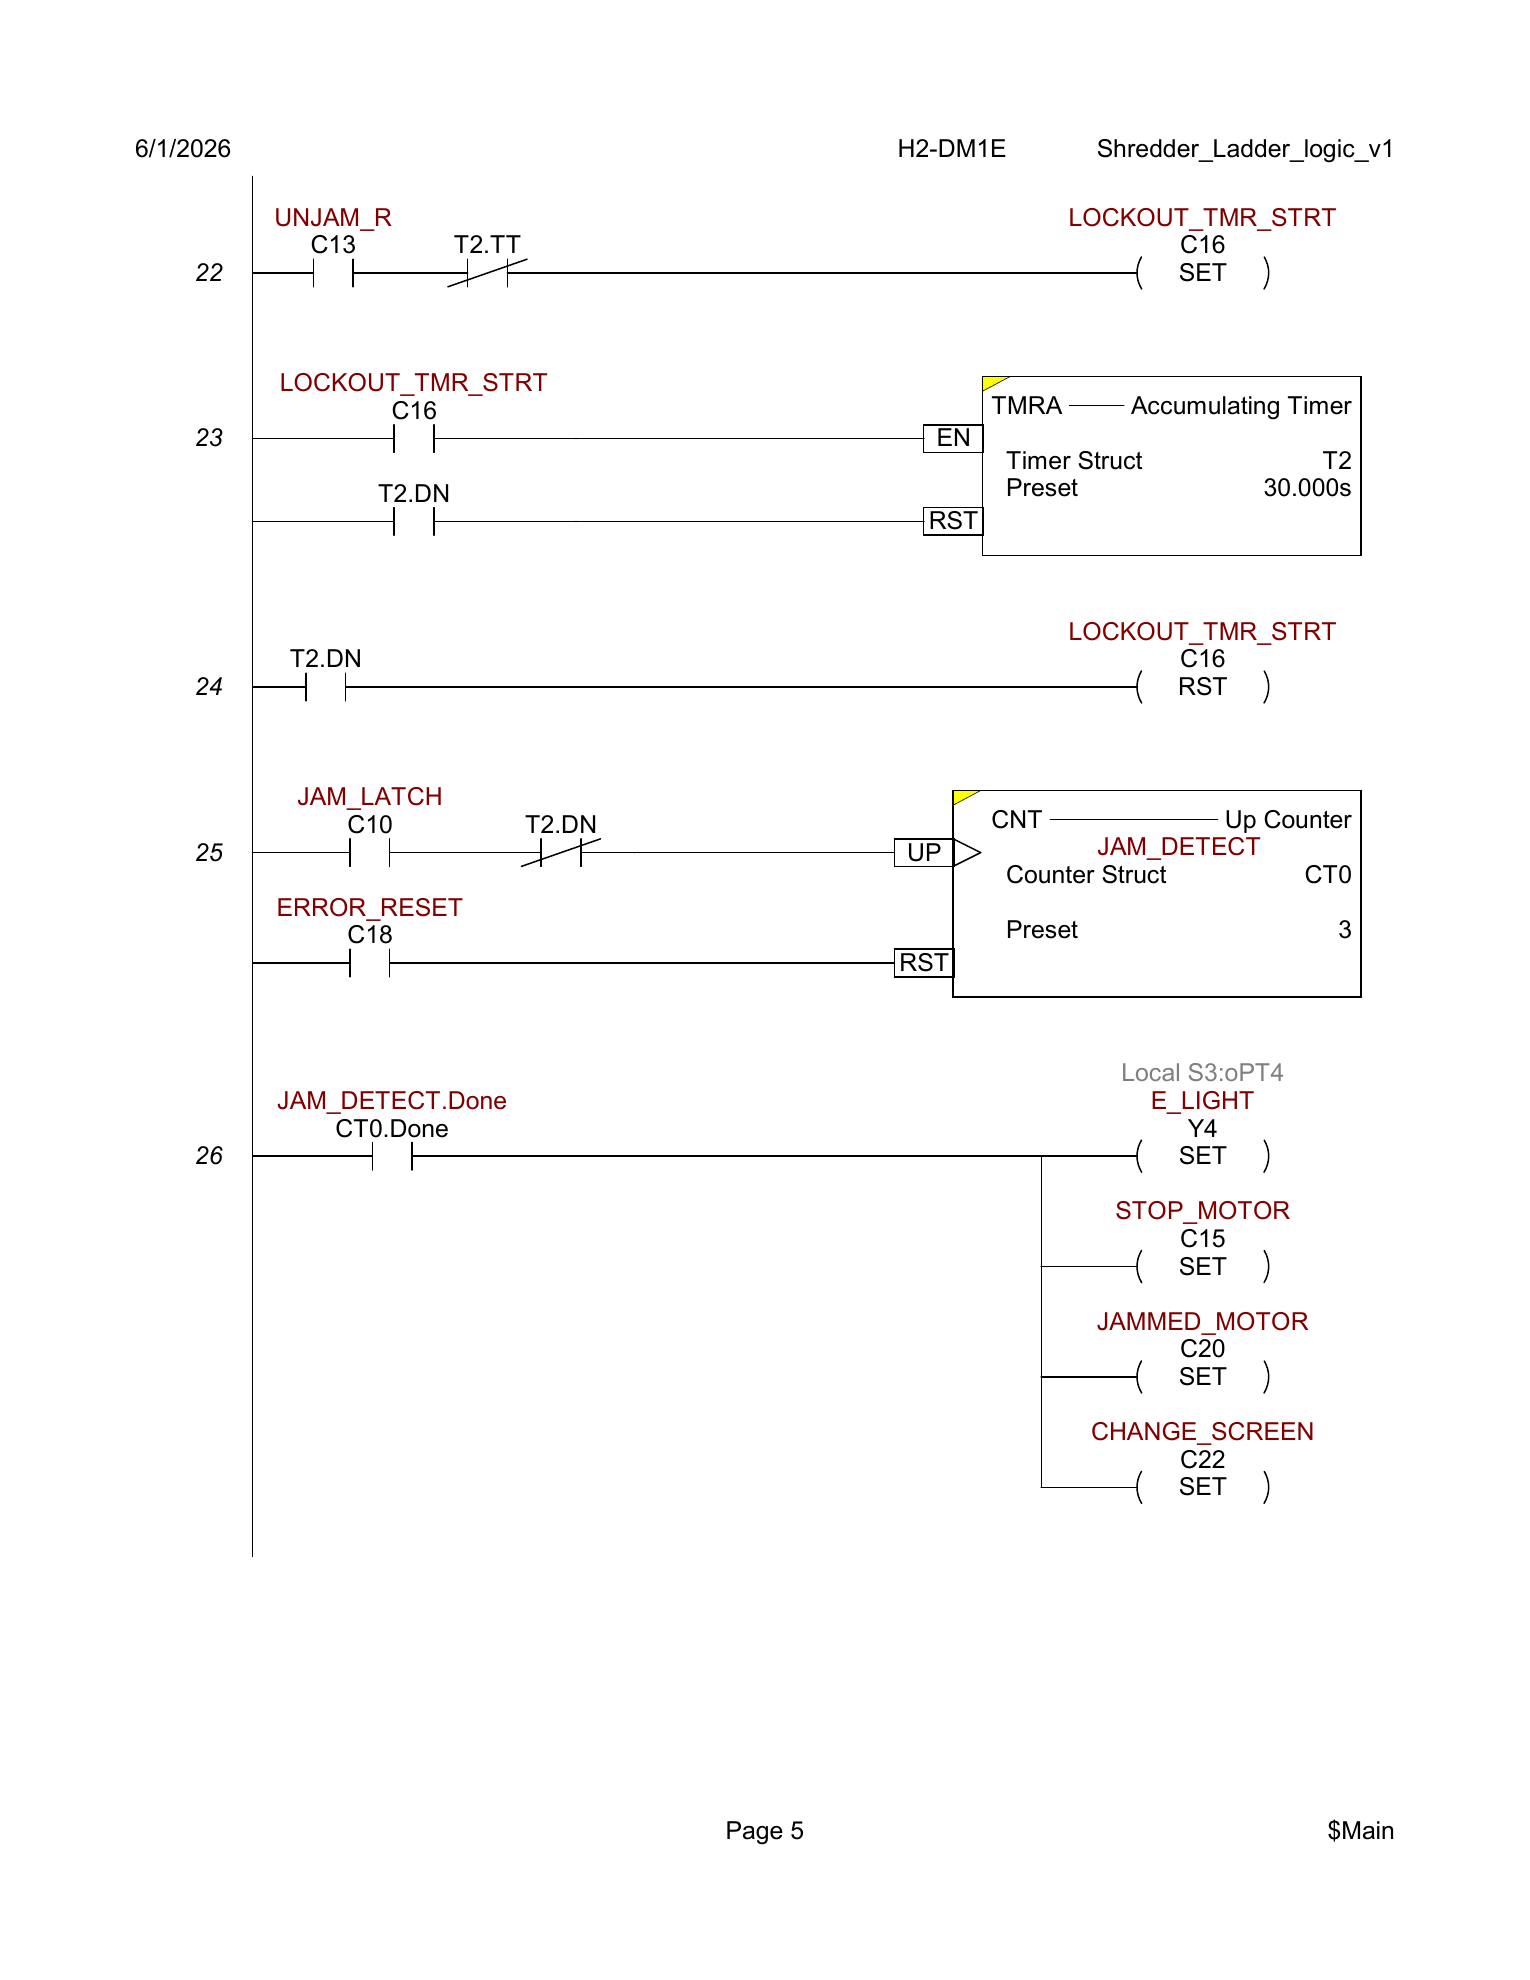
\includegraphics[height=6.5in]{./Pictures/Ladder_5.png}\hspace{3pt}%
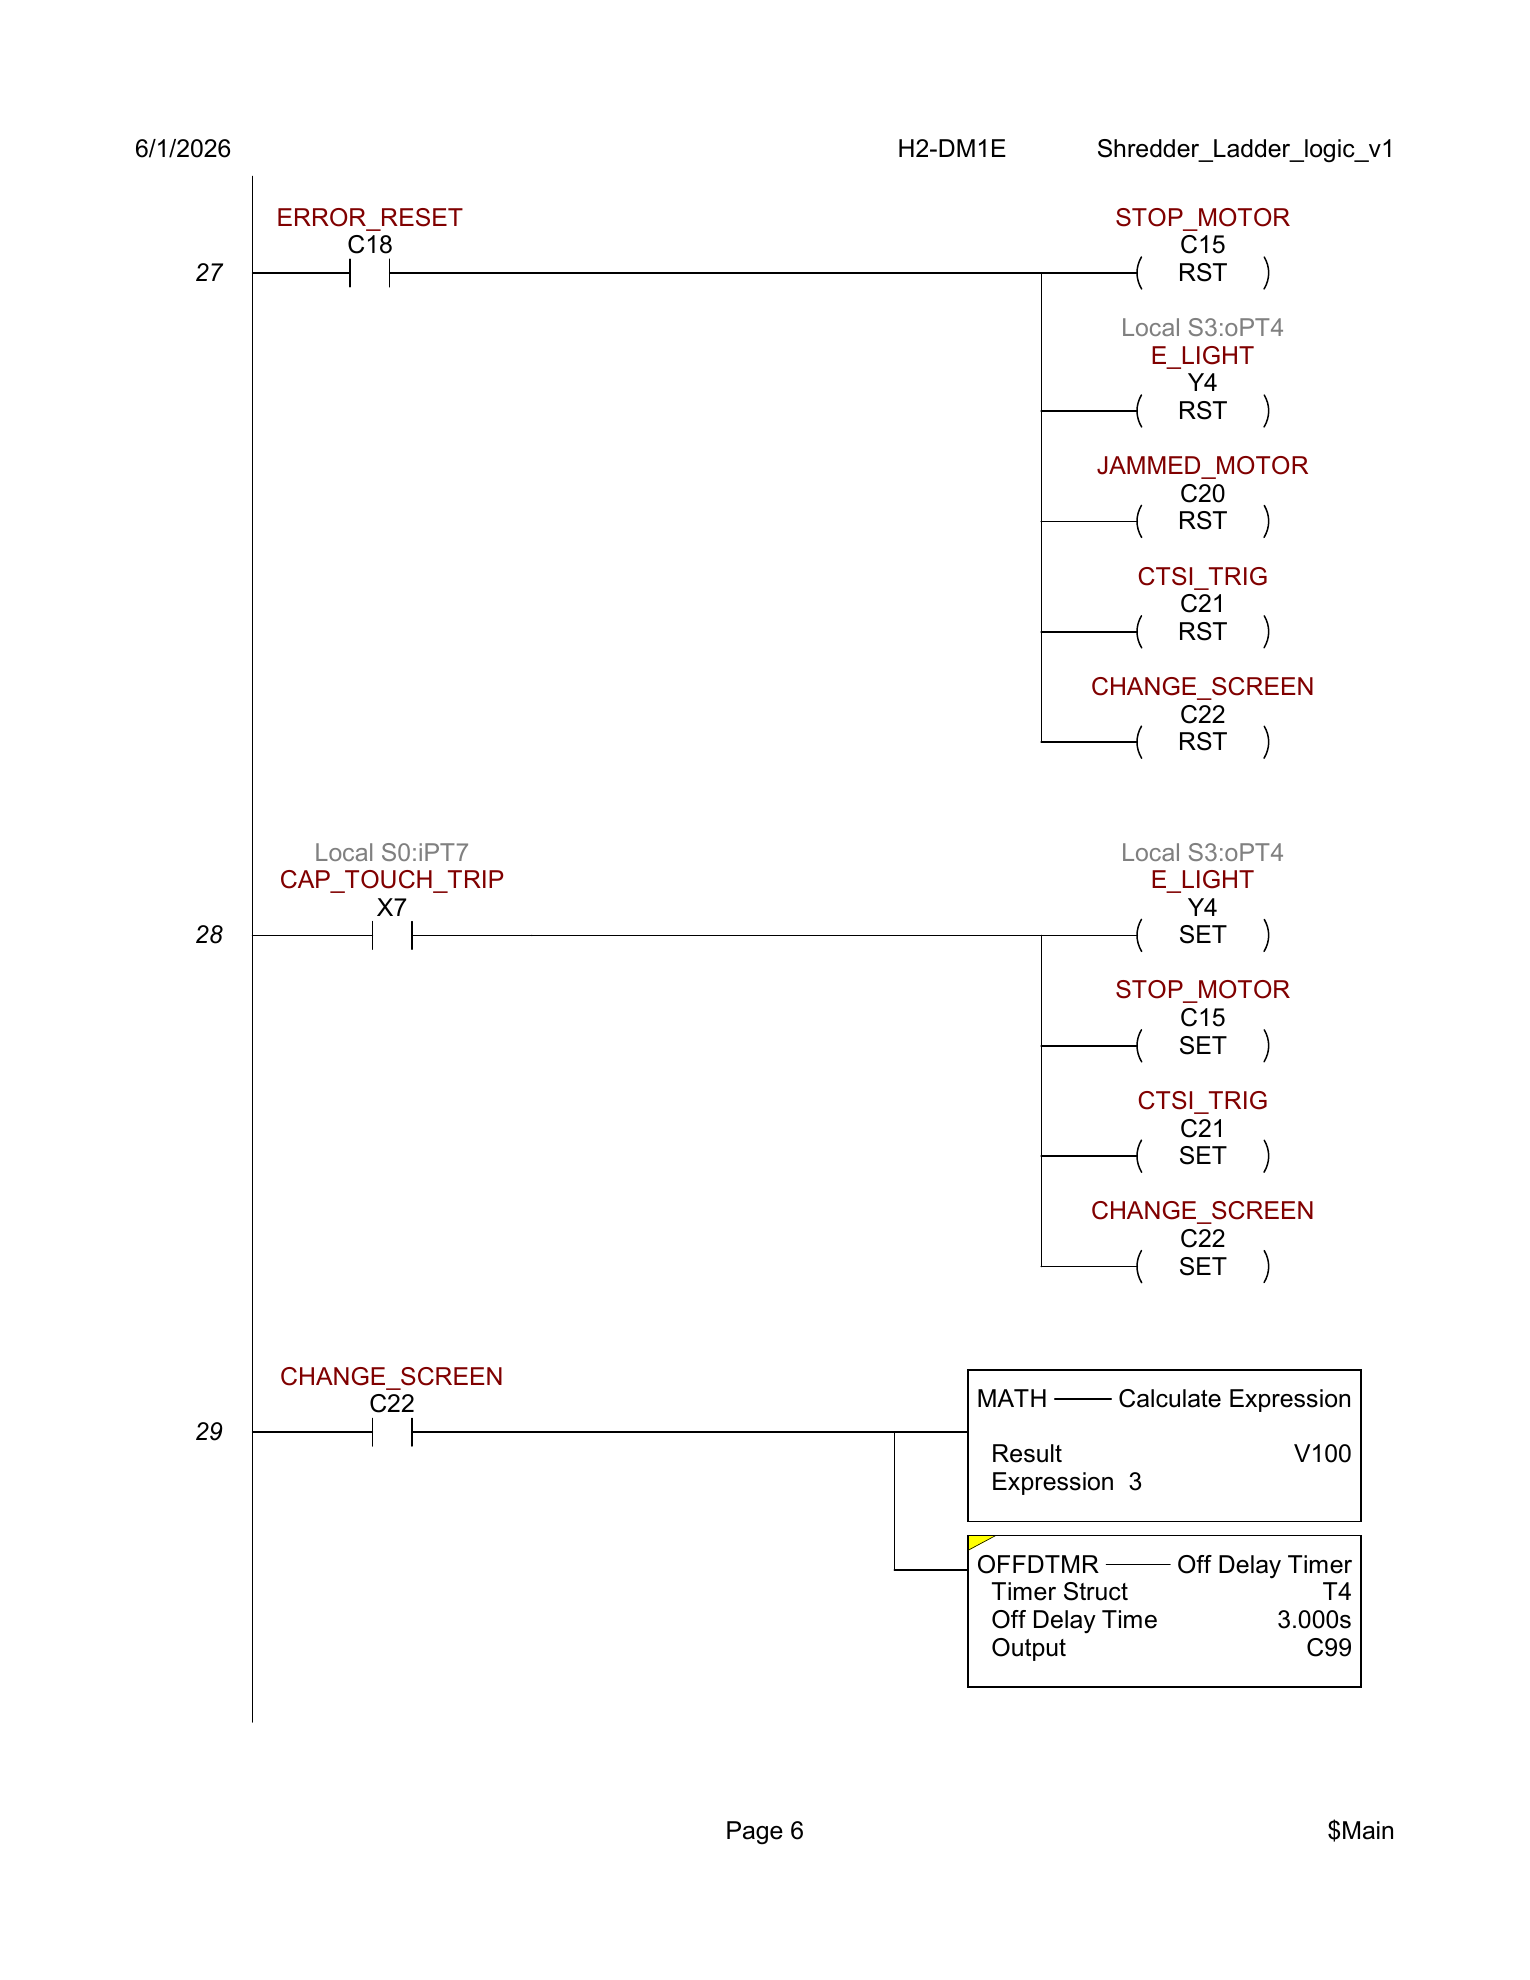
\includegraphics[height=6.5in]{./Pictures/Ladder_6.png}\hspace{3pt}%
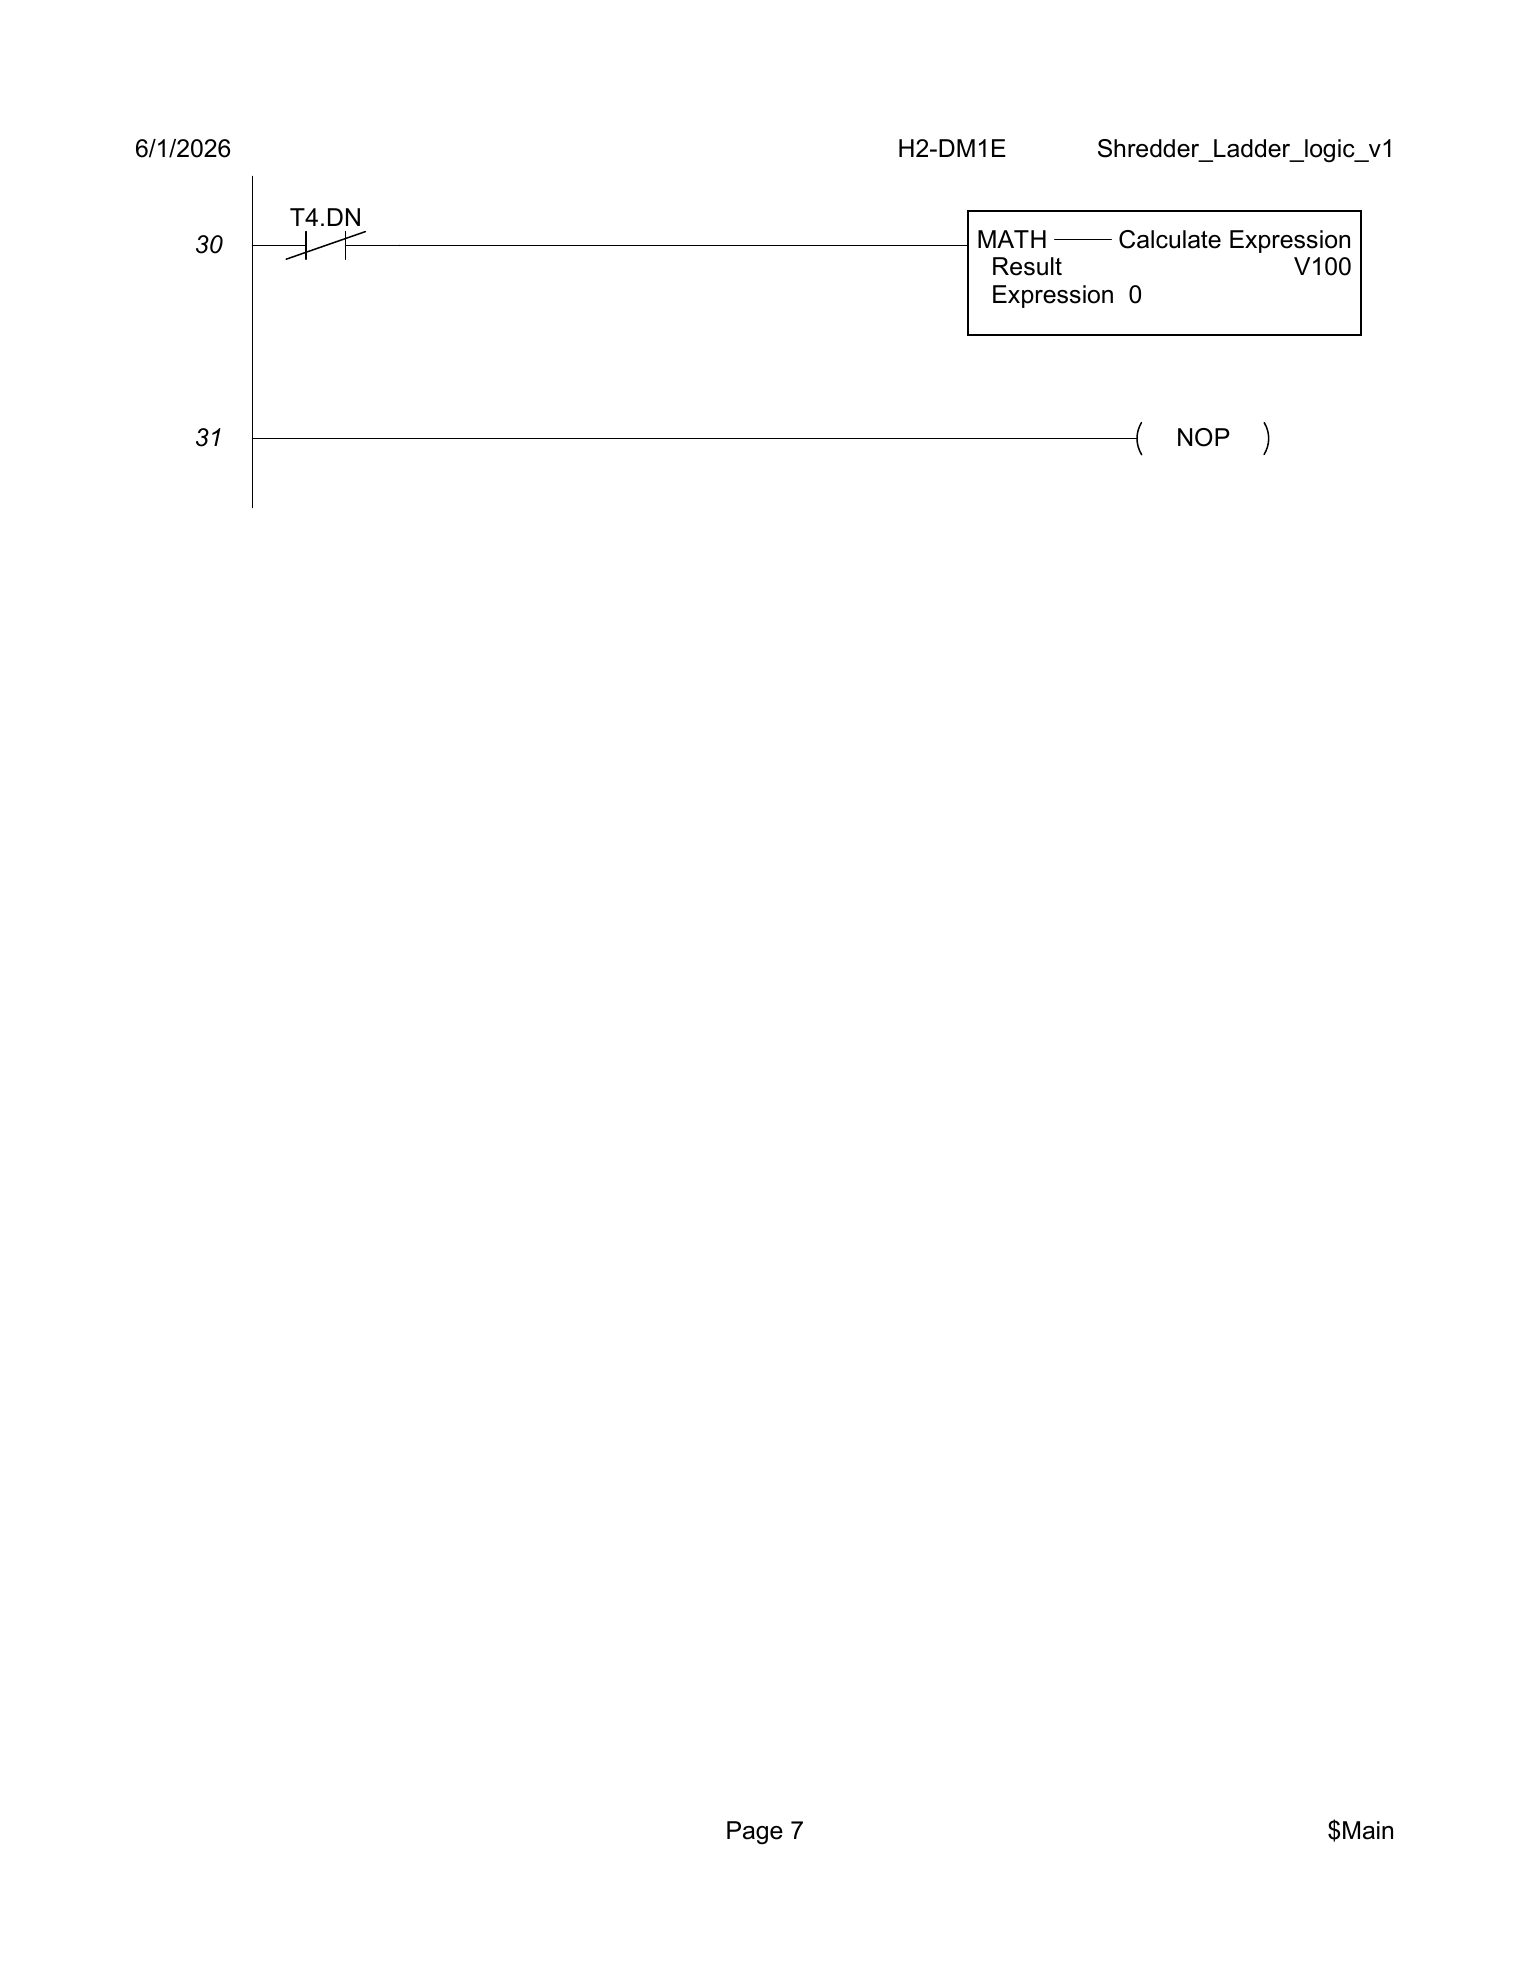
\includegraphics[height=6.5in]{./Pictures/Ladder_7.png}\\[2pt]
{\small\itshape Pages 1--7: init \textbullet\ run gating \textbullet\ indicators \textbullet\ E-stop / jam \textbullet\ lockout + counter \textbullet\ fault reset \textbullet\ end.}
\end{minipage}

% ============== BOTTOM FEATURE STRIP ==============
% Four equal-width info cards pushed down to sit flush against the
% bottom margin so the page has equal whitespace on every side.
\vfill
\noindent
\newcommand{\statbox}[2]{%
  \begin{tcolorbox}[
    enhanced, sharp corners, boxrule=0pt, frame hidden,
    interior style={top color=PSUcream, bottom color=white},
    borderline north={4pt}{0pt}{PSUgreen},
    left=14pt, right=14pt, top=10pt, bottom=12pt,
    width=\linewidth, height=2.6in,
    fontupper=\sffamily\normalsize,
    title=#1, coltitle=PSUgreen,
    fonttitle=\sffamily\bfseries\large,
    attach title to upper={\par\smallskip},
  ]
  #2
  \end{tcolorbox}}
\begin{minipage}[t]{0.243\textwidth}
\statbox{Project By the Numbers}{%
\textbf{31} ladder rungs in production.\\[3pt]
\textbf{27} HMI tags across 4 screens.\\[3pt]
\textbf{14} component sheets in the point list.\\[3pt]
\textbf{3} strikes before the motor locks out.\\[3pt]
\textbf{2 s} unjam reverse stroke.\\[3pt]
\textbf{150\%} over-torque threshold on the VFD.\\[3pt]
\textbf{\$969.88} spent against the \textbf{\$1{,}000} control-panel budget (\textbf{\$30.12} under).\\[3pt]
\textbf{Lots} of ``no, lowballer -- I know what I got'' from vendors during procurement.}
\end{minipage}\hfill
\begin{minipage}[t]{0.243\textwidth}
\statbox{Hardware Stack}{%
\textbf{PLC:} DirectLOGIC 205 + H2-DM1E.\\[3pt]
\textbf{HMI:} C-more EA1-T4CL.\\[3pt]
\textbf{VFD:} Huanyang HY02D211B-T.\\[3pt]
\textbf{Motor:} IronHorse MTCP2-002 (2 HP, 1735\,RPM, 145TC, TEFC, VFD-rated).\\[3pt]
\textbf{PSU:} Mean Well NDR-480-24.\\[3pt]
\textbf{Contactor:} Mitsubishi SD-N35.}
\end{minipage}\hfill
\begin{minipage}[t]{0.243\textwidth}
\statbox{Future Work}{%
Production motor selection (3--5\,HP) supersedes \texttt{PD141--PD144}.\\[3pt]
Mechanical integration and full shred-load run pending -- ME team did not deliver the prototype by end of term.\\[3pt]
Capacitive-touch (CTSI) module on \texttt{X7}: machine-level verification pending.\\[3pt]
Modbus link to the VFD for richer telemetry (deferred -- the Modbus module exceeded the \$1{,}000 control-panel budget, so the analog \texttt{VO} / \texttt{VI} path was used instead).}
\end{minipage}\hfill
\begin{minipage}[t]{0.243\textwidth}
\statbox{Acknowledgments}{%
Thanks to \textbf{Bridget Lannigan} (MME / Ichor Systems) for sponsoring the project; to advisors \textbf{Prof.~Andrew Greenberg}, \textbf{Dr.~Jonathan Bird}, and \textbf{Robert Paxton}; to the \textbf{ME capstone team} for the mechanical design and ongoing integration coordination; and to the \textbf{PSU Power Engineering Laboratory} for bench access.\\[6pt]
\textit{ECE 412/413 Capstone Poster Session $\bullet$ PSU MCECS $\bullet$ June 12, 2026}}
\end{minipage}

\end{document}
